%% VIth_SPHERIC_paper_tempalte.tex
%% V1.0
%% 2003/03/20
%% by Benedict Rogers
%% courtesy of nicolas.grenier@ec-nantes
%% courtesy of pierre.maruzewski@epfl.ch
%%
%% NOTE: This text file uses MS Windows line feed conventions. When (human)
%% reading this file on other platforms, you may have to use a text
%% editor that can handle lines terminated by the MS Windows line feed
%% characters (0x0D 0x0A).

% Note that the a4paper option is mainly intended so that authors in
% countries using A4 can easily print to A4 and see how their papers will
% look in print. Authors are encouraged to use U.S.
%
% Also note that the "draftcls" or "draftclsnofoot", not "draft", option
% should be used if it is desired that the figures are to be displayed in
% draft mode.
%
% This paper can be formatted using the peerreviewca
% (instead of conference) mode.
\documentclass[a4paper,conference]{IEEEtran}
% If the IEEEtran.cls has not been installed into the LaTeX system files,
% manually specify the path to it:
% \documentclass[conference]{../sty/IEEEtran}

% Dimensions of margins (DO NOT MODIFY THEM)
\setlength{\textheight}    {23.4cm}%
\setlength{\topmargin}     {-0.8cm}%
\setlength{\headheight}    {0.6cm}%
\setlength{\headsep}       {0.9cm}%

% some very useful LaTeX packages include:

\usepackage{cite}      % Written by Donald Arseneau
                        % V1.6 and later of IEEEtran pre-defines the format
                        % of the cite.sty package \cite{} output to follow
                        % that of IEEE. Loading the cite package will
                        % result in citation numbers being automatically
                        % sorted and properly "ranged". i.e.,
                        % [1], [9], [2], [7], [5], [6]
                        % (without using cite.sty)
                        % will become:
                        % [1], [2], [5]--[7], [9] (using cite.sty)
                        % cite.sty's \cite will automatically add leading
                        % space, if needed. Use cite.sty's noadjust option
                        % (cite.sty V3.8 and later) if you want to turn this
                        % off. cite.sty is already installed on most LaTeX
                        % systems. The latest version can be obtained at:
                        % http://www.ctan.org/tex-archive/macros/latex/contrib/supported/cite/

\usepackage{graphicx}  % Written by David Carlisle and Sebastian Rahtz
                        % Required if you want graphics, photos, etc.
                        % graphicx.sty is already installed on most LaTeX
                        % systems. The latest version and documentation can
                        % be obtained at:
                        % http://www.ctan.org/tex-archive/macros/latex/required/graphics/
                        % Another good source of documentation is "Using
                        % Imported Graphics in LaTeX2e" by Keith Reckdahl
                        % which can be found as esplatex.ps and epslatex.pdf
                        % at: http://www.ctan.org/tex-archive/info/
% NOTE: for dual use with latex and pdflatex, instead load graphicx like:
%\ifx\pdfoutput\undefined
%\usepackage{graphicx}
%\else
%\usepackage[pdftex]{graphicx}
%\fi

% However, be warned that pdflatex will require graphics to be in PDF
% (not EPS) format and will preclude the use of PostScript based LaTeX
% packages such as psfrag.sty and pstricks.sty. IEEE conferences typically
% allow PDF graphics (and hence pdfLaTeX). However, IEEE journals do not
% (yet) allow image formats other than EPS or TIFF. Therefore, authors of
% journal papers should use traditional LaTeX with EPS graphics.
%
% The path(s) to the graphics files can also be declared: e.g.,
% \graphicspath{{../eps/}{../ps/}}
% if the graphics files are not located in the same directory as the
% .tex file. This can be done in each branch of the conditional above
% (after graphicx is loaded) to handle the EPS and PDF cases separately.
% In this way, full path information will not have to be specified in
% each \includegraphics command.
%
% Note that, when switching from latex to pdflatex and vice-versa, the new
% compiler will have to be run twice to clear some warnings.


%\usepackage{psfrag}    % Written by Craig Barratt, Michael C. Grant,
                        % and David Carlisle
                        % This package allows you to substitute LaTeX
                        % commands for text in imported EPS graphic files.
                        % In this way, LaTeX symbols can be placed into
                        % graphics that have been generated by other
                        % applications. You must use latex->dvips->ps2pdf
                        % workflow (not direct pdf output from pdflatex) if
                        % you wish to use this capability because it works
                        % via some PostScript tricks. Alternatively, the
                        % graphics could be processed as separate files via
                        % psfrag and dvips, then converted to PDF for
                        % inclusion in the main file which uses pdflatex.
                        % Docs are in "The PSfrag System" by Michael C. Grant
                        % and David Carlisle. There is also some information
                        % about using psfrag in "Using Imported Graphics in
                        % LaTeX2e" by Keith Reckdahl which documents the
                        % graphicx package (see above). The psfrag package
                        % and documentation can be obtained at:
                        % http://www.ctan.org/tex-archive/macros/latex/contrib/supported/psfrag/

%\usepackage{subfigure} % Written by Steven Douglas Cochran
                        % This package makes it easy to put subfigures
                        % in your figures. i.e., "figure 1a and 1b"
                        % Docs are in "Using Imported Graphics in LaTeX2e"
                        % by Keith Reckdahl which also documents the graphicx
                        % package (see above). subfigure.sty is already
                        % installed on most LaTeX systems. The latest version
                        % and documentation can be obtained at:
                        % http://www.ctan.org/tex-archive/macros/latex/contrib/supported/subfigure/

%\usepackage{url}       % Written by Donald Arseneau
                        % Provides better support for handling and breaking
                        % URLs. url.sty is already installed on most LaTeX
                        % systems. The latest version can be obtained at:
                        % http://www.ctan.org/tex-archive/macros/latex/contrib/other/misc/
                        % Read the url.sty source comments for usage information.

%\usepackage{stfloats}  % Written by Sigitas Tolusis
                        % Gives LaTeX2e the ability to do double column
                        % floats at the bottom of the page as well as the top.
                        % (e.g., "\begin{figure*}[!b]" is not normally
                        % possible in LaTeX2e). This is an invasive package
                        % which rewrites many portions of the LaTeX2e output
                        % routines. It may not work with other packages that
                        % modify the LaTeX2e output routine and/or with other
                        % versions of LaTeX. The latest version and
                        % documentation can be obtained at:
                        % http://www.ctan.org/tex-archive/macros/latex/contrib/supported/sttools/
                        % Documentation is contained in the stfloats.sty
                        % comments as well as in the presfull.pdf file.
                        % Do not use the stfloats baselinefloat ability as
                        % IEEE does not allow \baselineskip to stretch.
                        % Authors submitting work to the IEEE should note
                        % that IEEE rarely uses double column equations and
                        % that authors should try to avoid such use.
                        % Do not be tempted to use the cuted.sty or
                        % midfloat.sty package (by the same author) as IEEE
                        % does not format its papers in such ways.

\usepackage{amsmath}   % From the American Mathematical Society
                        % A popular package that provides many helpful commands
                        % for dealing with mathematics. Note that the AMSmath
                        % package sets \interdisplaylinepenalty to 10000 thus
                        % preventing page breaks from occurring within multiline
                        % equations. Use:
%\interdisplaylinepenalty=2500
                        % after loading amsmath to restore such page breaks
                        % as IEEEtran.cls normally does. amsmath.sty is already
                        % installed on most LaTeX systems. The latest version
                        % and documentation can be obtained at:
                        % http://www.ctan.org/tex-archive/macros/latex/required/amslatex/math/



% Other popular packages for formatting tables and equations include:

%\usepackage{array}
% Frank Mittelbach's and David Carlisle's array.sty which improves the
% LaTeX2e array and tabular environments to provide better appearances and
% additional user controls. array.sty is already installed on most systems.
% The latest version and documentation can be obtained at:
% http://www.ctan.org/tex-archive/macros/latex/required/tools/

% Mark Wooding's extremely powerful MDW tools, especially mdwmath.sty and
% mdwtab.sty which are used to format equations and tables, respectively.
% The MDWtools set is already installed on most LaTeX systems. The lastest
% version and documentation is available at:
% http://www.ctan.org/tex-archive/macros/latex/contrib/supported/mdwtools/


% V1.6 of IEEEtran contains the IEEEeqnarray family of commands that can
% be used to generate multiline equations as well as matrices, tables, etc.


% Also of notable interest:

% Scott Pakin's eqparbox package for creating (automatically sized) equal
% width boxes. Available:
% http://www.ctan.org/tex-archive/macros/latex/contrib/supported/eqparbox/



% Notes on hyperref:
% IEEEtran.cls attempts to be compliant with the hyperref package, written
% by Heiko Oberdiek and Sebastian Rahtz, which provides hyperlinks within
% a document as well as an index for PDF files (produced via pdflatex).
% However, it is a tad difficult to properly interface LaTeX classes and
% packages with this (necessarily) complex and invasive package. It is
% recommended that hyperref not be used for work that is to be submitted
% to the IEEE. Users who wish to use hyperref *must* ensure that their
% hyperref version is 6.72u or later *and* IEEEtran.cls is version 1.6b
% or later. The latest version of hyperref can be obtained at:
%
% http://www.ctan.org/tex-archive/macros/latex/contrib/supported/hyperref/
%
% Also, be aware that cite.sty (as of version 3.9, 11/2001) and hyperref.sty
% (as of version 6.72t, 2002/07/25) do not work optimally together.
% To mediate the differences between these two packages, IEEEtran.cls, as
% of v1.6b, predefines a command that fools hyperref into thinking that
% the natbib package is being used - causing it not to modify the existing
% citation commands, and allowing cite.sty to operate as normal. However,
% as a result, citation numbers will not be hyperlinked. Another side effect
% of this approach is that the natbib.sty package will not properly load
% under IEEEtran.cls. However, current versions of natbib are not capable
% of compressing and sorting citation numbers in IEEE's style - so this
% should not be an issue. If, for some strange reason, the user wants to
% load natbib.sty under IEEEtran.cls, the following code must be placed
% before natbib.sty can be loaded:
%
% \makeatletter
% \let\NAT@parse\undefined
% \makeatother
%
% Hyperref should be loaded differently depending on whether pdflatex
% or traditional latex is being used:
%
%\ifx\pdfoutput\undefined
%\usepackage[hypertex]{hyperref}
%\else
%\usepackage[pdftex,hypertexnames=false]{hyperref}
%\fi
%
% Pdflatex produces superior hyperref results and is the recommended
% compiler for such use.



% *** Do not adjust lengths that control margins, column widths, etc. ***
% *** Do not use packages that alter fonts (such as pslatex).         ***
% There should be no need to do such things with IEEEtran.cls V1.6 and later.


% correct bad hyphenation here
\hyphenation{op-tical net-works semi-conduc-tor IEEEtran}


\usepackage{fancyheadings}
\usepackage{float}
\usepackage{afterpage}
\usepackage{subfig}
\pagestyle{fancy}

\lhead{$9^{th}$ international SPHERIC workshop}
\rhead{Paris, France, June, 03-05 2014}
\cfoot{} % to avoid page numbering

\newcommand{\OF}{OpenFOAM\textsuperscript{\textregistered}}
\newcommand{\FF}{Fluent\textsuperscript{\textregistered}}
\newcommand{\tauB}{\underline{\underline{\boldsymbol{\tau}}}}
\newcommand{\vv}{\mathbf{v}}
\newcommand{\xx}{\mathbf{x}}
\newcommand{\aaa}{\mathbf{a}}
\newcommand{\ww}{\mathbf{w}}
\newcommand{\gb}{\mathbf{g}}
\newcommand{\nn}{\mathbf{n}}
\newcommand{\yy}{\mathbf{y}}
\newcommand{\Mat}{Matlab{\small$^{\textregistered}$}}


\begin{document}

% paper title
\title{p-FEM }


% author names and affiliations
% use a multiple column layout for up to three different
% affiliations
\author{\IEEEauthorblockN{Authors Name/s per 1st Affil.}
\IEEEauthorblockA{line 1 (of Affiliation): dept. name of organization\\
line 2: name of organization, acronyms acceptable\\
line 3: City, Country\\
line 4: e-mail address if desired}
\and
\IEEEauthorblockN{Authors Name/s per 2nd Affil.}
\IEEEauthorblockA{dept. name of organization\\
name of organization\\
City, Country\\
e-mail address if desired}
\and
\IEEEauthorblockN{Authors Name/s per 3rd Affil.}
\IEEEauthorblockA{dept. name of organization\\
name of organization\\
City, Country\\
e-mail address if desired}}

% use only for invited papers
%\specialpapernotice{(Invited Paper)}

% make the title area
\maketitle

\begin{abstract}
This electronic document is a ``live'' template. The various components of your paper [title, text, heads, etc.] are already defined on the style sheet, as illustrated by the portions given in this document.
\end{abstract}




\section{Introduction}

%Las formulaciones estándar para la solución de las ecuaciones de fenómenos de transporte pueden ser agrupadas en dos categorías, dependiendo del enfoque seleccionado para describir los términos inerciales. En el enfoque Euleriano la aceleración es descripta como la suma de una derivada espacial de la velocidad más un término convectivo. El segundo grupo pertenece a las formulaciones Lagrangianas en dónde la aceleración es simplemente descripta como una derivada total (o derivada material) de la velocidad.

%Durante los últimos treinta años, la simulación de flujo de fluidos incompresibles ha sido principalmente basada en la formulación Euleriana de las ecuaciones fluido-dinámicas sobre dominios fijos\cite{Donea03}. Por otro lado, las formulaciones Lagrangianas justifican su popularidad resolviendo flujos de superficie libre o complicados flujos de fluidos de diferentes propiedades intensivas (multi-fluídos), en los cuales el enfoque Euleriano estándar es impreciso o, en ciertos casos, imposible de usar.

Particle methods have started to combine the Lagrangian part with a grid that fixed or re-meshed every k time steps supports part of the pressure and velocity calculation. The original idea given by Monaghan \cite{Mon77} or later works applied to fluid mechanics \cite{Monaghan88} where a pure Lagrangian perspective was used during the whole meshless computation has been in some cases completed using other well known discretization methods as FVM \cite{Quinlan} or FEM \cite{Calvo}. We could try to find the first combination of Lagrangian methods and FEM methods in the paper \cite{Ide03b} where a extended Delaunay Tesellation is used to reconstruct the mesh while the fluid evolves. In this method known as MFEM, the construction of the shape functions inside each polyhedron is based on a non-Sibsonian interpolation.

The next step in this evolution was the first version of the PFEM method \cite{Idelsohn04}, which was a robust method designed to solve fluid–structure interaction problems including free surface, breaking waves, flow separations, etc...where lagrangian particles and meshing processes are alternated with the advantage of having a FEM structure that supports the differential equation solvers. An interesting difference between the PFEM and other particle methods as SPH or MPM \cite{Wieckowsky04} is that the mesh particles do not transport mass and consequently have a volume, in contrast PFEM uses non material points that transport fluid properties with fixed density. 

Other methods that also combine both Eulerian and Lagrangian perspectives are the arbitrary Eulerian-Lagrangian (ALE)\cite{Donea83} methods or the semi-Lagrangian methods \cite{Bermejo}. The Lagrangian perspective makes possible to use a material derivative formulation where the absence of the non linear convective terms transform the Navier-Stokes system into a transformed linear coupled problem. Methodologies like the backward Characteristics method \cite{Bermejo} gives also this possibility but if the process is done in a fixed mesh without any distortion, a diffusion process appears due to the interpolation of the feet of characteristics.

Most of the methods cited before including PFEM have a uncomfortable drawback which is the necessity of constructing or controlling the mesh quality during the simulation if an accuracy of the solution has to be maintained. The evaluation of the mesh distortions or the re-meshing processes are always computationally expensive and it would be interesting exploring the possibility of avoiding that step. Consequently a new generation of the PFEM methodology could be developed in such a way that no re-meshing is necessary.
In contrast to the backward characteristic method where the feet of the characteristic line was searched and located in a mesh element based on the known velocity fields at past time steps, a new strategy known as X-IVAS (eXplicit Integration following the Velocity and Acceleration Streamlines)\cite{Idelsohn12}. This methodology uses the streamlines at the present time step instead of the the particle trajectories to convect the fluid particles. The use of this strategy on a fixed mesh and interpolate the particle information to the mesh nodes gives a new improved method known as PFEM-2\cite{Idelsohn12b}. The use of particles give the possibility of solving complex accurate flows with large time steps, while the fixed mesh allows accurate solutions of the fractional step method without any remeshing process. Mesh nodes and moving particles interchange information using interpolation processes using different strategies. A detailed explanation of the PFEM-2 method is given in Section \ref{PFEM_Algorithm}.

In this work the PFEM-2 has been used to solve free surface flows in different problems starting from classical benchmark problems as the lid driven cavity and finishing with problems of industrial interest. As in most of the FEM derived methodologies the introduction of a complex geometry is not a problem. The treatment of the free surface has been done simulating both fluids that share the interface and using a scalar function to identify each fluid. To improve the pressure calculation along the free surface different versions of the enrichment technique \cite{Coppola} has been used. The computation of the free surface at different positions has been performed and compared to other well reputed and commercial Eulerian codes with good results but using larger time steps with any loss of numerical stability. 

  
\section{PFEM Algorithm}\label{PFEM_Algorithm}

Everything is known at time $n$. Subindexes $()_j$ y $()_p$ represents all nodes and particles respectively. Let $\phi$ and $\psi$ the pressure and velocity basis functions.

\begin{enumerate}
  \item Acceleration Stage: Calculate acceleration on the mesh nodes.


  \begin{equation}\label{Step1a}
\int_{\Omega}\mathbf{a}^{n}_{\tau}\psi_j d\Omega=\int_{\Omega}\mu \nabla^{2}\mathbf{v} \psi_j d\Omega=-\int_{\Omega}\mu \nabla\mathbf{v} \nabla \psi_j d\Omega + \int_{\Gamma}\mu \nabla\mathbf{v} \psi_j d\Omega
\end{equation}

\begin{equation}\label{Step1b}
\int_{\Omega}\mathbf{a}^{n}_{p}\psi_j d\Omega=-\int_{\Omega}\nabla p \psi_j d\Omega=\int_{\Omega} p \nabla \psi_j d\Omega - \int_{\Gamma} p \psi_j d\Omega
\end{equation}

\begin{equation}\label{Step1c}
\mathbf{a}^{n}=\mathbf{a}^{n}_{p} + (1-\theta)\mathbf{a}^{n}_{\tau}
\end{equation}

Multifluids $\theta=1$ y $p^n=0$

  \item X-IVAS Stage: Evaluate new particle position and intermediate velocity following frozen fields

  \begin{equation}\label{Step2a}
\mathbf{x}^{n+1}_{p}=\mathbf{x}^{n}_{p} + \int_{n}^{n+1} \mathbf{v}^{n}(\mathbf{x}^{\alpha}_{p}) \ d\alpha
\end{equation}

\begin{equation}\label{Step2b}
\widehat{\widehat{\mathbf{v}}}^{n+1}_{p}=\mathbf{v}^{n}_{p} + \int_{n}^{n+1} \mathbf{a}^{n}(\mathbf{x}^{\alpha}_{p}) + \mathbf{f}^{\alpha} (\mathbf{x}^{\alpha}_{p})  \ d\alpha
\end{equation}

  \item Projection Stage: Project velocity and level set function from particles to the mesh:
  \begin{equation}\label{Step3a}
\displaystyle \widehat{\widehat{\mathbf{v}}}^{n+1}_{j}=\frac{\sum_{p} \mathbf{v}^{n+1}_{p} W(\mathbf{x}_{j}-\mathbf{x}_{p})}{\sum_{p} W(\mathbf{x}_{j}-\mathbf{x}_{p})}
\end{equation}

\begin{equation}\label{Step3b}
\displaystyle \lambda^{n+1}_{j}=\frac{\sum_{p} \lambda^{n+1}_{p} W(\mathbf{x}_{j}-\mathbf{x}_{p})}{\sum_{p} W(\mathbf{x}_{j}-\mathbf{x}_{p})}
\end{equation}

  \item Implicit Viscosity Stage: Implicit correction of the viscous diffusion with FEM:

 \begin{equation}\label{Step4a}
\displaystyle \widehat{\mathbf{v}}^{n+1}_{j}=\widehat{\widehat{\mathbf{v}}}^{n+1}_{j} + \theta \Delta t \mathbf{a}^{n+1}_{\tau}
\end{equation}

 \item Poisson Stage: Search the pressure value solving the Poisson equation system with FEM:
 \begin{equation}\label{Step5a}
  \ \nabla \cdot [\frac{\Delta t}{\rho}\nabla(\delta p^{n+1})] = \nabla \cdot \widehat{\mathbf{v}}_j^{n+1}
 \end{equation}

 \item Correction Stage: Update the mesh and particle velocity with pressure and diffusion corrections:
 \begin{equation}\label{Step6a}
  \int_{\Omega} \rho_j \mathbf{v}_j^{n+1}\ d\Omega \ = \ \int_{\Omega} \rho_j  \widehat{\mathbf{v}}_j^{n+1}\ d\Omega\ - \int_{\Omega} \Delta t \ (\mathbf{a}_j^{n+1} - \mathbf{a}_j^{n})\ d\Omega
 \end{equation}
  \begin{equation}\label{Step6b}
  \rho_p \mathbf{v}_p^{n+1}\  = \ \rho_p \widehat{\widehat{\mathbf{v}}}_p^{n+1} + \sum_{j} \delta \mathbf{v}_j^{n+1} \psi_j(\mathbf{x}_{p})
  \end{equation}
  where $\delta \mathbf{v}_j^{n+1} = \mathbf{v}_j^{n+1}-\widehat{\widehat{\mathbf{v}}}_j^{n+1}$.

%  \item 
%  \item 
%  \item 
\end{enumerate}

\section{Second order improvements.}


The well known \textit{Brezzi-BabÃŒska} condition (also called \textit{inf-sup} condition) determinates the interpolation families for the velocity and pressure to ensure stability and convergence in the Stokes problem. Originally, the PFEM-2 method uses the family P1/P1 (linear triangular elements) to approximate the variables $\mathbf{u}$ and $p$ on the mesh\cite{Idelsohn12b}. % because is a computationally cheap approach.
However, this family does not satisfy the \textit{inf-sup} condition, then it is unstable, so it requires to use stabilization at the Poisson step. Maybe carrying on the extra cost of the stabilization is possible, but using linear elements does not provided good accuracy with coarser meshes. Using finer meshes in PFEM-2 introduce another extra cost due to the necessity for use more particles to approximate the fields and update nodal values.

An alternative proposal is presented in this report. The idea is using the called Taylor-Hood finite elements\cite{HoodTaylor73}, which are presented in Figure \ref{fg:taylor-hood}. They consist on a quadratic approximation for the velocity and continuous linear approximation for pressure (family P2/P1). It is demonstrated that this family is stable because it satisfies the \textit{inf-sup} condition. However, that advantage could not be useful if the cpu-time required to reach some accuracy is larger than using P1/P1 elements.

\begin{figure}[htbp]
  \begin{center}
      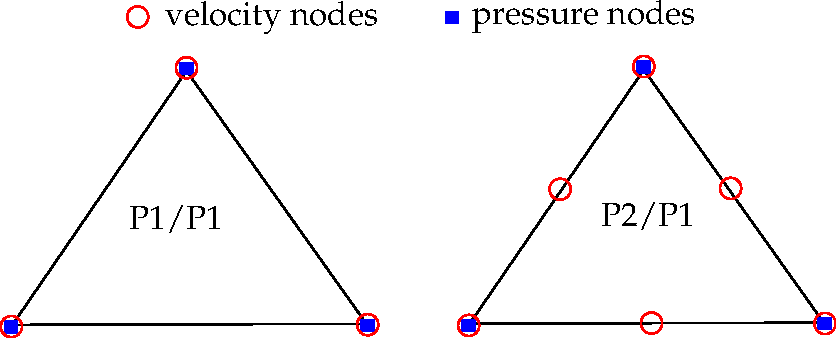
\includegraphics[width=.9\columnwidth]{images/taylor_hood.pdf}
  \end{center}
  \caption{\label{fg:taylor-hood} Left: Family P1/P1 originally used by PFEM-2. Right: Family P2/P1 proposed by this work.}
\end{figure}

\subsection{Square Cavity Tests}
% Previously, a new strategy to assemble the matrices and vectors of the linear equation systems was developed. It consists of pre-assembling the global matrices at the beginning of the simulation (for example mass and stiffness matrices), and after, at each time-step performing the final assemble with matrix-vector products. This approach improves the efficiency of the previous code (which assemble the matrices doing a loop over all the elements each time-step) in about a 20\%. However, it remains testing problems with variable coefficients.

% As we will see later, this approach is not useful for multi-fluids simulations, because the elemental matrices must be assembled each time-step and that formulation depends on the fluid zone that the element represents (interface zone or not).

Cartesian meshes were used for all cases. The name of the meshes indicates how many vertex-nodes there are in x-direction and y-direction respectly. For example the mesh \texttt{50x50-1ºorder} has 50 vertex-nodes in x-axis and 50 vertex-nodes in y-axis, conforming around 4800 first order triangular elements with 2500 degrees of freedom per variable. With second order grids have similar criteria, for example \texttt{25x25-2ºorder} has 25 vertex-nodes in each direction conforming 1250 second order triangular elements with approximately 2601 degrees of freedom per variable. Therefore the equation systems to solve with those meshes have approximately the same size.

\subsubsection{Re1000}

It was simulated using $\Delta t = 0.02$. Final simulation time $t_{final} = 50[s]$.

\begin{figure}[htbp]
  \begin{center}
      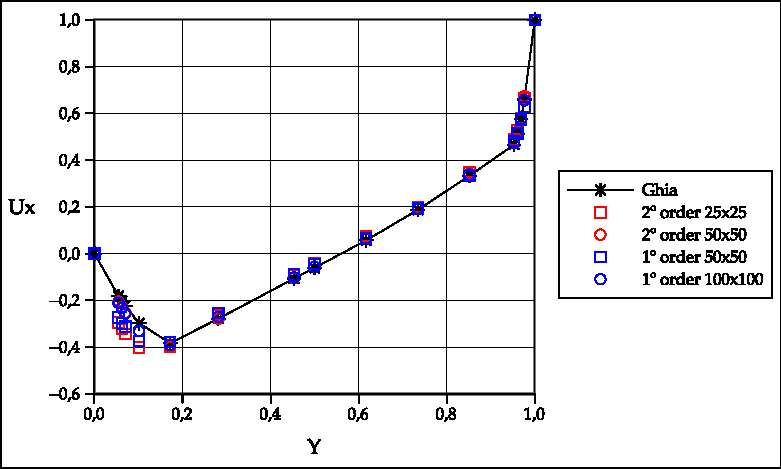
\includegraphics[width=.85\linewidth]{images/Re_1000_Ux.pdf}
      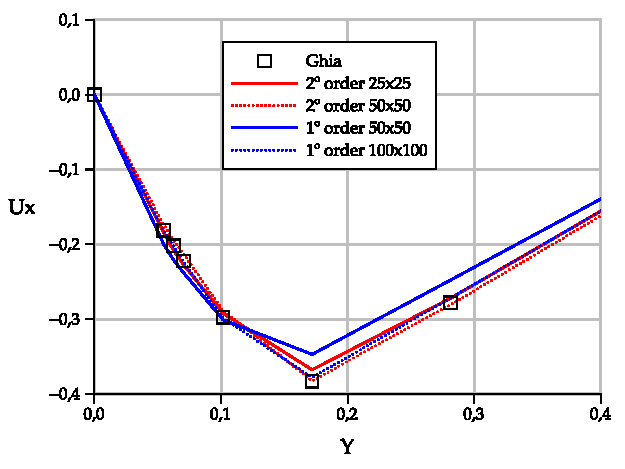
\includegraphics[width=.85\linewidth]{images/Re_1000_Ux_zoom.pdf}
  \end{center}
  \caption{\label{fg:Re1000u} Comparison with Ghia References at $Re=1000$. $u$ velocities at x-centerline.}
\end{figure}

\begin{figure}[htbp]
  \begin{center}
      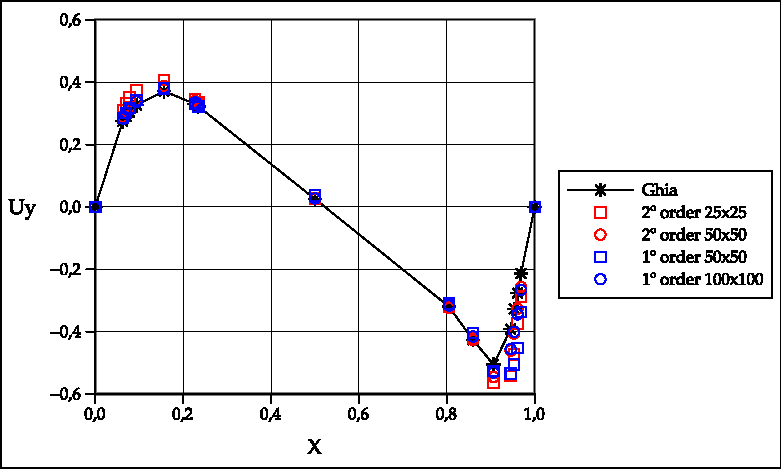
\includegraphics[width=.85\linewidth]{images/Re_1000_Uy.pdf}
      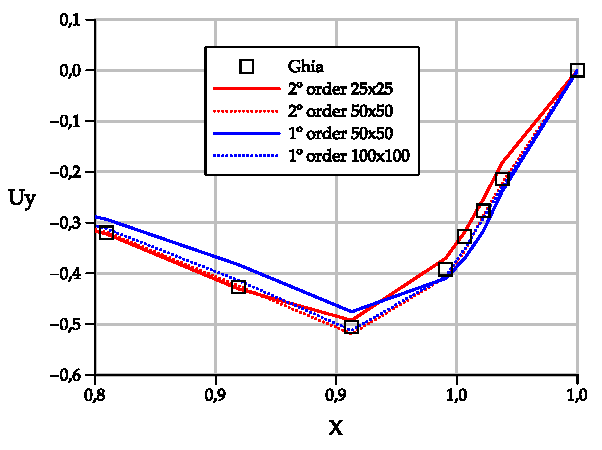
\includegraphics[width=.85\linewidth]{images/Re_1000_Uy_zoom.pdf}
  \end{center}
  \caption{\label{fg:Re1000v} Comparison with Ghia References at $Re=1000$. $v$ velocities at y-centerline.}
\end{figure}

\begin{table}[htbp]
\begin{center}
{\footnotesize
\begin{tabular}[h]{||c|c|c|c|c||}
    \hline
      Stage & $25x25$ - 2º order & $50x50$  - 2º order & $50x50$ - 1º order & $100x100$ - 1º order\\
      \hline
      \hline
	Acceleration & 34.6[s]& 134.58[s]& 22.8[s] & 97.9\\
	X-IVAS & 102.3[s]& 423.7[s]& 108.93[s] & 488.9 \\
	Projection & 32.4[s]& 153.8[s]& 75.0[s] & 359.1\\
	Poisson & 48.3[s]& 190.4[s]& 66.4[s] & 278.7\\
	Correction & 39.9[s]& 190.0[s]& 39.7[s] & 233.6\\
      \hline
	TOTAL & 257.57[s]& 1092.6[s]& 312.9[s] & 1458.1\\
      \hline
      \hline
	RMS $u$ & $2.0\times10^{-3}$ & $1.4\times10^{-3}$ & $5.8\times10^{-3}$ & $1.7\times10^{-3}$ \\
	RMS $v$ & $3.0\times10^{-3}$ & $2.2\times10^{-3}$ & $6.7\times10^{-3}$ & $2.4\times10^{-3}$ \\
      \hline
      \hline
\end{tabular}
}
\caption{\label{Tabla:times_Re_1000} Comparison table for CPU-times for the different PFEM-2 stages and the root mean square of the approximation error of $u$ and $v$. Case: $Re=1000$.}
\end{center}
\end{table}

\newpage

\subsubsection{Re 3200}


It was simulated using $\Delta t = 0.01$. Final simulation time $t_{final} = 100[s]$.

\begin{figure}[htbp]
  \begin{center}
      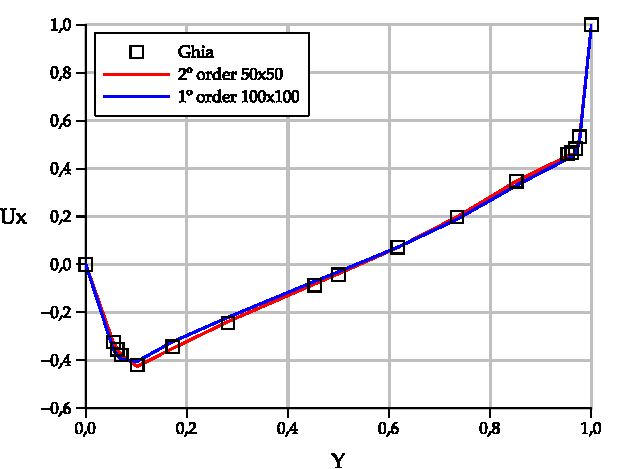
\includegraphics[width=.85\linewidth]{images/Re_3200_Ux.pdf}
      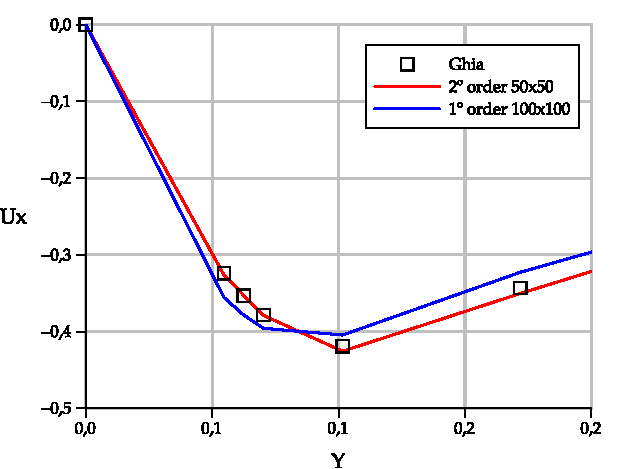
\includegraphics[width=.85\linewidth]{images/Re_3200_Ux_zoom.pdf}
  \end{center}
  \caption{\label{fg:Re3200} Comparison with Ghia References at $Re=3200$. $u$ velocities at x-centerline.}
\end{figure}

\begin{table}[htbp]
\begin{center}
{\footnotesize
\begin{tabular}[h]{||c|c|c||}
    \hline
      Stage & $50x50$  -2º order & $100x100$ - 1º order\\
      \hline
      \hline
	Acceleration & 134.9[s]& 98.01[s]\\
	X-IVAS & 427.5[s]& 499.9[s] \\
	Projection & 154.7[s]& 368.5\\
	Poisson & 191.1[s]& 283.6\\
	Correction & 189.2[s]& 242.9\\
      \hline
	TOTAL & 1097.4[s]& 1492.9\\
      \hline
      \hline
	RMS $u$ & 0.0106 & 0.0113 \\
      \hline
      \hline
\end{tabular}
}
\caption{\label{Tabla:times_Re_3200} Comparison table for CPU-times (to achieve $30[s]$ of real time) for the different PFEM-2 stages. Also the root mean square of the approximation error of $u$ at the end of the simulation is presented. Case: $Re=3200$.}
\end{center}
\end{table}

\newpage

\subsubsection{Re 10000}


It was simulated using $\Delta t = 0.01$. Final simulation time $t_{final} = 75[s]$.

\begin{figure}[htbp]
  \begin{center}
      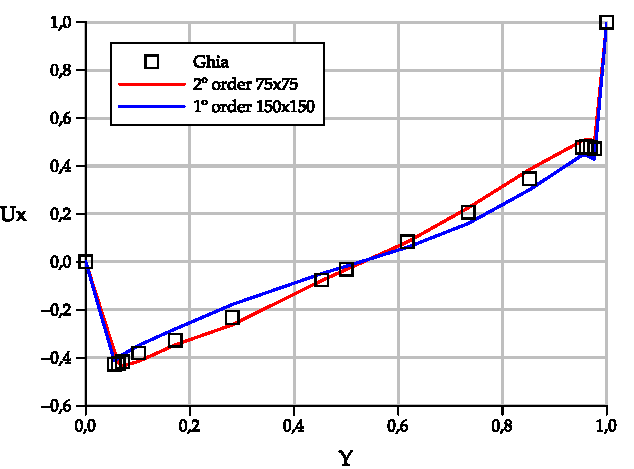
\includegraphics[width=.85\linewidth]{images/Re_10000_Ux.pdf}
  \end{center}
  \caption{\label{fg:Re10000} Comparison with Ghia References at $Re=10000$. $u$ velocities at x-centerline.}
\end{figure}


\begin{table}[htbp]
\begin{center}
{\footnotesize
\begin{tabular}[h]{||c|c|c||}
    \hline
      Stage & $75x75$  -2º order & $150x150$ - 1º order\\
      \hline
      \hline
	Acceleration & 515.0[s]& 367.1[s]\\
	X-IVAS & 1741.2[s]& 2114.1[s] \\
	Projection & 731.5[s]& 1651.2[s]\\
	Poisson & 740.9[s]& 1078.6[s]\\
	Correction & 911.4[s]& 1237.9[s]\\
      \hline
	TOTAL & 4640.0[s]& 6449.0[s]\\
      \hline
      \hline
	RMS $u$ & 0.015 & 0.0213 \\
      \hline
      \hline
\end{tabular}
}
\caption{\label{Tabla:times_Re_10000} Comparison table for CPU-times for the different PFEM-2 stages and the root mean square of the approximation error of $u$. Case: $Re=10000$.}
\end{center}
\end{table}

\newpage

\subsection{Summary}

  \begin{itemize}
   \item With the same number of nodes, second order achieve better accuracy than first order.
   \item With the same number of nodes, second order might be more efficient (it requires less elements and, then, less particles).
   \item The conclusion about the efficiency is only applicable to incompressible homogeneous flows with constant parameters (viscosity, density, etc). However, that asseveration can be modified when problems with non-constant diffusion-matrices will be required (turbulence modeling, multi-fluids. etc). Also several tests have demonstrated that the matrix storage is only useful for small or medium problems, but it is not applicable to large problems (more than 1M elements) because in those cases, it is slower than the traditional elemental assemble at each time step.
  \end{itemize}

\section{Free surface flows improvements}.

There are several, but no large, differences between the PFEM-2 algorithm for homogeneous flows and the multi-fluids version. Those differences are due to a density jump appears and it is necessary to include strategies to capture correctly the interface between the fluids. Most of the details presented in this section have been reported in \cite{Idelsohn13c}, however we consider the reinforcement of those issues is relevant.

Taking into account the Algorithm presented in section \ref{PFEM_Algorithm}, next are considerations to manage and improve each one of the stages for the particular case of multifluids problems. 

\subsection{Internal interfaces tracking}

The accurate and efficient simulation of interface evolution is of fundamental importance in the simulation of multiphase flows. It is essential that the interface remains sharp and can fold, break and merge. Large jumps of fluid density and viscosity across the interface need to be properly taken into account in order to satisfy the momentum balance at the vicinity of the interface. 

Methods used to describe the evolution of interfaces can be clustered in two classes, namely: interface capturing and interface tracking methods. While in the former the interface is determined by an implicit function that is advected in a Eulerian frame (see Volume of Fluid \cite{VoF} and Level Set\cite{Osher01}), in the latter the interface evolution equation is solved in a Lagrangian fashion, for example by evolving marker particles.

The spatial domain discretization using mesh and particles allows PFEM2 to select an appropriate combination of those approaches. Each high-density (e.g. water) particle is marked as positive ($\lambda_p=1$) and each low-density (e.g. air) is colored as negative ($\lambda_p=-1$). This value is advected adding one equation to the \textit{Streamline Integration Stage}: $\frac{D\lambda}{Dt}=0$,i.e. each particle only keeps its marker value during the entire simulation. 

The last means, for instance, that even if a water particle is momentarily on an air regime, it will remain as a water particle for further determination of the interface position. However, in that case and because the most similar path to the real trajectory of the particle is desired, the particle leaves the streamlines and follows a trajectory defined by the acting forces, being the simplest one the parabolic motion (only gravity force) or coupled with a water droplet drag model.
 
After \textit{Projection Stage}, each node $j$ has a distance function-like value $\lambda_j$ which is used to determinate the instantaneous local interface inside each element. That zone is defined by an iso-line (an iso-plane in 3D) where $\lambda(\xx)=0$

\subsection{Shape function enrichments for pressure gradient discontinuity capturing}

In typical finite element methods, the gradient of the shape functions $\nabla\phi_j$ are continuous within each element, and therefore any unknown interpolated is also continuous. When the interface crosses an element the discontinuity in the material properties leads to discontinuities in the gradients of the unknowns that the interpolation used cannot capture. For the case of two different density fluids the interpolation errors in the pressure give rise to spurious velocities that can render the solution meaningless.

In order to improve the approximation, an enriched space has been used for the pressure gradients based on the one presented by Coppola [36]. This new degree of freedom is statically condensed within each element in the pressure equation and then recovered in the correction step. In this manner, the number of unknowns remains constant in time and, therefore, the system matrix does not have to be rebuilt at each time step, which is an expensive task due to memory allocation.  The gradient enrichment is illustrated in Fig. 5.3a.
On the other hand, a new enrichment function has been developed to account for pressure discontinuities. The function (Figure 5.3b) ensures a constant jump across the interface, which allows us to account for the effect of surface tension. Despite that has not been employed in the examples presented in this work, the effectiveness of combining the two enrichments functions has been validated for scalar diffusion and Stokes problems with discontinuities by comparing the results against conforming meshes [41]

  In order to capture properly the jump of the pressure gradient on the interface between the fluids, the enrichment proposed by Coppola-Owen and Codina\cite{Coppola05} is used.

  Briefly, the main idea is to enrich the finite element space for the pressure in the elements cut by the interface. This is done including a new shape function $N^*$ that has a constant gradient on each side of the interface, its value is zero at the element nodes and is $C^0$ continuous in the element. Figure \ref{fg:enrichment} presents a graphical description of this new shape function.


  \begin{figure}[H]
  \centering
    \subfloat[]{
	  \label{fg:enrichment1}         %% Etiqueta para la primera subfigura
	  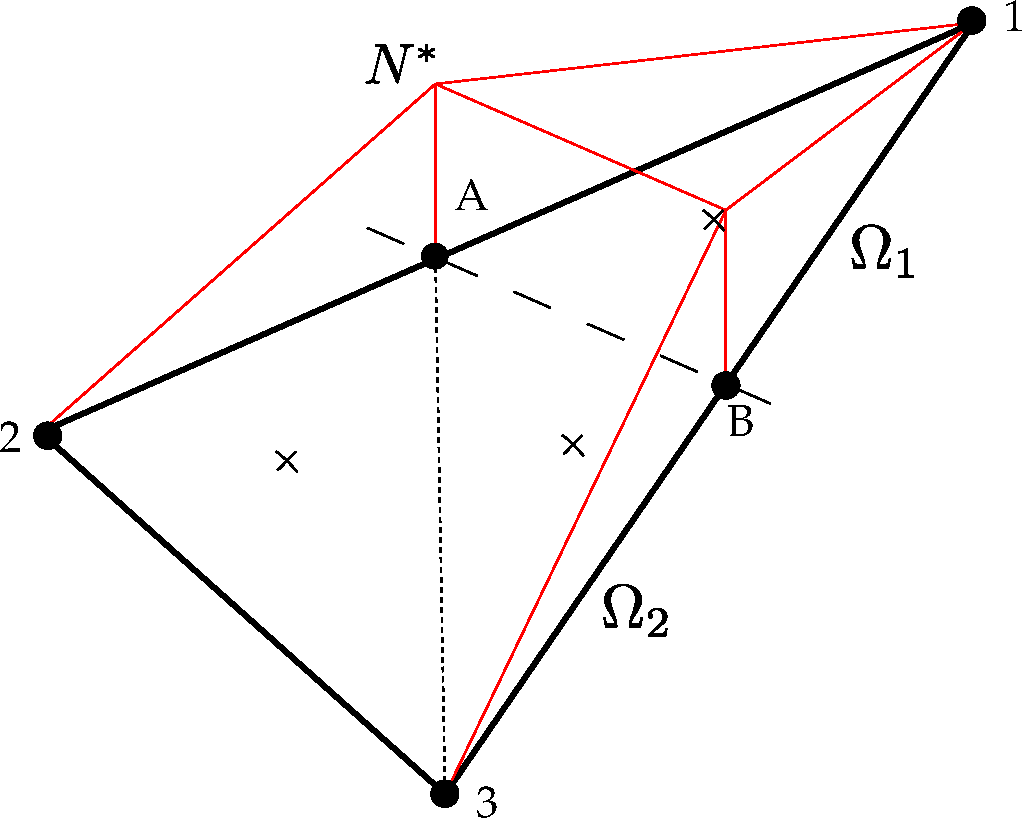
\includegraphics[width=.49\columnwidth]{images/enrichment1.pdf}
    }
    %%----segunda subfigura----
    \subfloat[]{
	  \label{fg:enrichment2}         %% Etiqueta para la segunda subfigura
	  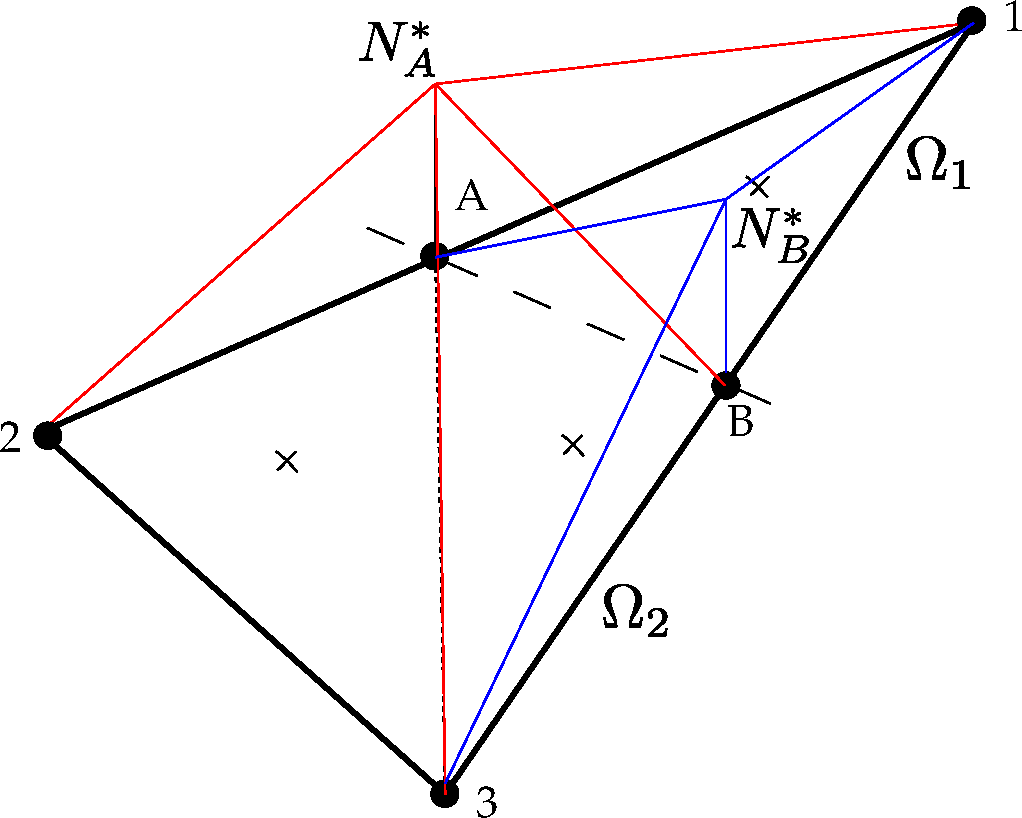
\includegraphics[width=.49\columnwidth]{images/enrichment2.pdf}
    }
   \caption{2D Enrichment functions. Figure \ref{fg:enrichment1} shows an enrichment using only one enrichment function $N^*$ which $N^*(\xx_A)=1$ and $N^*(\xx_1)=N^*(\xx_2)=N^*(\xx_3)=0$. Figure \ref{fg:enrichment2} presents the enrichment functions which are constructed following $N_A^*(\xx_A)=1$,$N_B^*(\xx_B)=1$ and $N_A^*(\xx_1)=N_A^*(\xx_2)=N_A^*(\xx_3)=N_A^*(\xx_B)=N_B^*(\xx_1)=N_B^*(\xx_2)=N_B^*(\xx_3)=N_B^*(\xx_A)=0$ .}
   \label{fg:enrichment}                %% Etiqueta para la figura entera
\end{figure}

   Therefore, the pressure is now interpolated in the cut element following:

   \begin{equation}
      p_h(\xx) = \sum_{i=1}^{nnodes} (N_i(\xx) \ p_i) + N^*(\xx) \ p^*
   \end{equation}

   where $N_i$ are the traditional linear shape functions, and $N^*$ is defined as a linear combination of them (Equations \ref{N_enrichment-2} and \ref{N_enrichment-1}),

   \begin{align}
    N^*|_{\Omega_2} = & \ k_1 N_1 \label{N_enrichment-2}\\
    N^*|_{\Omega_1} = & \ k_2 N_2 + k_3 N_3 \label{N_enrichment-1}
   \end{align}
   where $k_1 = \dfrac{\psi_2-\psi_1}{\psi_2}$, $k_2 = \dfrac{\psi_1-\psi_2}{\psi_1}$ and $k_3 = -k_1\dfrac{\psi_3\psi_1}{\psi_3-\psi_1}$
	
	
   In order to capture the discontinuities and take advantage of the enrichment functions used, the integration rules need to be modified in elements cut by the front. The method we use is to divide each triangular element into up to three triangular sub elements. For each sub element the same integration rule as for the non-cut elements is used. Figure \ref{fg:enrichment}  shows that partition and the crosses represents the Gauss points for the integration. When using enrichment functions for the pressure, the material properties $\rho$,$\mu$ are taken as $\rho_1$,$\mu_1$ or $\rho_2$,$\mu_2$, depending on which part of the domain ($\Omega_1$ or $\Omega_2$) the integration point is found.

   \subsection{Pressure Iterations}

Most of multi-fluid flows present a large jump in the density properties, for instance water and air. For those cases, introducing a special strategy in the iterative algorithm to obtain acceptable convergence rates is mandatory. For instance, the strategy to introduce the last time step pressure field as the initial value for the first iteration of the next time step is not the best one. This is caused by the fact that the particles can move across several elements and through the interface during a time step (Figure 5.1) and, therefore, the pressure gradient of the previous time step would introduce a poor and even unstable approximation of the pressure forces.

Therefore, at each time-state, the value of the pressure is set to zero in order to avoid large errors in the evaluation of the pressure gradients in the initial value of the iterative process. As consequence of that, the acceleration over the particle only is due to viscous force and gravity force (pressure gradient is considered null) for this step.

    We are following the most similar path to the real trajectory of the particle. For the case of a water particle on water zones, we consider that the water streamlines are the best option. But on air zones, if the particle follows the air streamlines, poor approximations to the real trajectory will be obtained. Therefore, in the last situation, the water particle leaves the streamline and follows a trajectory defined by the acting forces, being the simplest one the parabolic motion (only gravity force) or coupled with a water droplet drag model.

    
\subsection{Enrichment for pressure gradient discontinuity capturing}

\subsection{Pressure Stage}

  The Poisson equation for the pressure appears after applying the divergence operator to
  \begin{equation}
    \vv^{n+1}\  = \ \hat \vv^{n+1} - \dfrac{\Delta t}{\rho} \ [\nabla (\delta p)]^{n+1}
    \label{correction_cont}
  \end{equation}

  which remains
  \begin{equation}
   \dfrac{\Delta t}{\rho} \ \nabla \cdot [\nabla(\delta p^{n+1})] = \nabla \cdot \hat \vv_j^{n+1}
  \end{equation}

  integrating, weighting with local shape functions and weakening, we can obtain the elemental contribution
  \begin{equation}
   [\Delta t \int_{\Omega^e} \frac{1}{\rho} \nabla N^T \nabla N \ d\Omega] \delta p^{n+1} = [\int_{\Omega^e} \nabla N^T \phi \ d\Omega] \hat \vv_j^{n+1}
  \end{equation}

  The main advantage of the above proposed enrichment shape functions is that the added degree of freedom is local to the element cut by the interface and can therefore be condensed after the element matrix has been computed and before assembly.

  Therefore, if the element is not cut by the interface, the traditional lineal shape functions are used for weighting and the variables are approximated in terms of that space: $\delta p^{n+1}(\xx) = \sum_i N_i(\xx) \delta p^{n+1}_i$ and $\hat{\vv}^{n+1}(\xx) = \sum_i \phi_i(\xx) \hat{\vv}^{n+1}_i$, being $\phi_i = N_i$.

  On the other hand, if the element is cut by the interface, we choose $N = [N_1; N_2; N_3; N^*]$ as weight shape functions and to approximate the pressure field (keeping only the traditional shape functions $\phi = [N_1; N_2; N_3]$ to approximate the velocity field). Then, for the split elements, the system before the condensation is:

  \begin{equation*}
   \begin{pmatrix}
      L_{std} & L_{std}^*\\
      {L_{std}^*}^T & L^*
   \end{pmatrix}\;
    \begin{pmatrix}
      \delta p^{n+1}\\
      p^*
   \end{pmatrix}\; = \;
   \begin{pmatrix}
      D_{std}\\
      D^*
   \end{pmatrix}\;
   (\hat{\vv}^{n+1})
   \label{poisson}
\end{equation*}

where
\begin{itemize}
 \item ${(L_{std})}_{ij} = \Delta t \int_{\Omega^e} \dfrac{1}{\rho} \nabla N_i^T \nabla N_j \ d\Omega$ with $[i,j] = 1,2,3$ (size [$3$x$3$])
 \item ${(L_{std}^*)}_{i} = \Delta t \int_{\Omega^e} \dfrac{1}{\rho} \nabla N_i^T \nabla N^* \ d\Omega$ with $i = 1,2,3$ (size [$3$x$1$])
 \item $L^* = \Delta t \int_{\Omega^e} \dfrac{1}{\rho} \nabla {N^*}^T \nabla N^* \ d\Omega$ (size [$1$x$1$])
 \item ${(D_{std})}_{ij} = \int_{\Omega^e} \nabla N_i^T \phi_j \ d\Omega$ with $[i,j] = 1,2,3$ (size [$3$x$3$])
 \item ${(D^*)}_{j} = \int_{\Omega^e}  \nabla {N^*}^ \phi_j \ d\Omega$ with $j = 1,2,3$ (size [$1$x$3$])
\end{itemize}

  Therefore, the system is statically condensed obtaining:

  \begin{equation}
   [L_{std} - L_{std}^*\frac{1}{L^*}{L_{std}^*}^T](\delta p^{n+1}) = [D_{std}- L_{std}^*\frac{1}{L^*}D^*](\hat{\vv}^{n+1})
   \label{condensing}
  \end{equation}

  If we are interested in solving the system in absolute pressure terms, the final system is

  \begin{equation}
  [L_{std} - L_{std}^*\frac{1}{L^*}{L_{std}^*}^T](p^{n+1}) = [D_{std}- L_{std}^*\frac{1}{L^*}D^*](\hat{\vv}^{n+1}) + [L_{std} - L_{std}^*\frac{1}{L^*}{L_{std}^*}^T] (p^n)
   \label{condensing-abs}
  \end{equation}


\subsection{Correction Stage}

 This stage is typical from fractional steps. However, the new degree of freedom for the pressure, which was condensed previously, must be taken into account in this step to calculate the correct pressure gradient. Therefore, we must \textit{recover} $p^*$ doing:

  \begin{equation}
  {p^*}^{n+1} = \frac{1}{L^*}[D^* \hat{\vv}^{n+1} - {L_{std}^*}^Tp^{n+1} + {L_{std}^*}^Tp^{n} + L^*{p^*}^n]
  \label{recovering}
  \end{equation}

 Finally, the equation system presented in Equation \ref{correction} must be solved.

 \begin{equation}
  \int_{\Omega} N \rho \vv^{n+1} d\Omega = \int_{\Omega} N \rho \hat{\vv}^{n+1} d\Omega - \Delta t \ [\int_{\Omega} N_{std} \nabla p^{n+1} d\Omega + \int_{\Omega} N^* \nabla p* d\Omega]
  \label{correction}
 \end{equation}

 Besides the nodal velocity correction, it also must be done the correction over particles. Must be noted this correction is done projecting the variation of the nodal velocity.
	
  \begin{equation}
    \rho_p \vv_p^{n+1}\  = \ \rho_p \hat \vv_p^{n+1} - \boldsymbol{\pi}^{-1}(\delta \vv_j^{n+1})
    \label{correction_particles}
  \end{equation}
  where $\delta \vv_j^{n+1} = \vv_j^{n+1} - \hat \hat \vv_j^{n+1}$.


\subsection{Iterations to improve the pressure-velocity coupling}

The initial value of the pressure iterations is set to zero in order to avoid large errors in the evaluation of the pressure gradients in the initial value of the iterative process. It must be noticed that despite this first iteration of the pressure calculation is
of first order, further iterations improve the incompressibility of the solution. Doing this implies that the stabilization effect of the first order fractional step is lost due to the higher order scheme. Tests with hundreds of iterations were performed and, effectively,
spurious pressure oscillations appear in the solution. However, for practical applications, only two or three iterations are needed in order to obtain pressure convergence and, despite not being theoretically stable, pressure oscillations do not appear in the solution. For this reason no stabilization technique is required in this case.

Another justification because the pressure is restarted each time step is that we can not predict accurately the value of ${p^*}^n$ on Equation \ref{recovering} at the first iteration (using the latest $p^*$ of the previous time-step may introduce several problems due to the movement of the interface). Therefore, the acceleration for the velocity in X-IVAS only can have the viscous forces.

%Detalle del tema de la inicialización a cero de la presión, fundamentalmente por el hecho de que hay dos fluidos. Citar el clindro, como caso donde a pesar de haber un sólo fluido el algoritmo de puesta a cero de la presión sigue siendo válido.


\section{Free surface results}


\subsection{Non-linear sloshing in a rectangular container}%Ansari

Free surface oscillations of a liquid confined in a closed container (sloshing phenomenon) are an important issue when big amounts of liquid are industrially transported. The phenomenon involves two fluids that share a free surface boundary separating them, normally the density of the upper fluid is several orders of magnitude less than the bottom one. This phenomenon has proven of great interest due to the fact that violent impacts of the fluid can affect the structural integrity of the container.

For the studied cases, the sloshing phenomenon is produced by a horizontal harmonic excitation $x = a_h (\sin \omega_h t)$, where $a_h$ is the excitation amplitude and $\omega_h$ is the excitation frequency of the rectangular tank where the two fluid phases are contained. The tank is divided in two parts, the bottom part is water with a density of $\rho_{I} = 1000 [kg/m^3]$ and the top part contains a fluid
with different densities $\rho_{II} = 1.3, 50, 200, 800 [kg/m^3]$, depending on the case studied\cite{Goni13}. The dimensions of the
tank are $a$(width) by $b$(height) and the initial free surface is at height $h$ from the bottom of the tank, see Figure \ref{fg:ansari-config}. The free surface starts the simulation as a horizontal line and is subsequently deformed by the tank excitation and the flow dynamics.

\begin{figure}[H]
  \begin{center}
      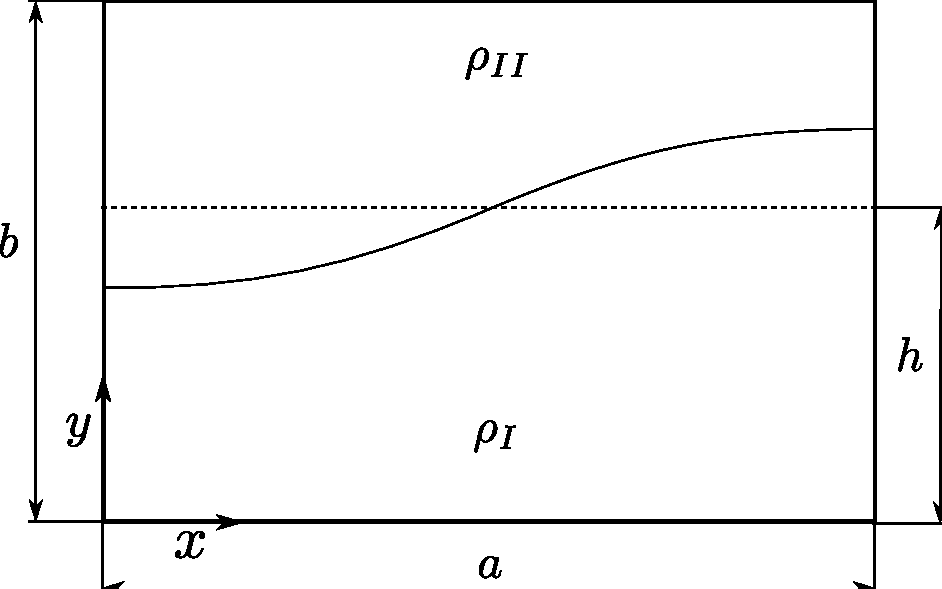
\includegraphics[width=.7\columnwidth]{images/ansari_config.pdf}
  \end{center}
  \caption{\label{fg:ansari-config} Configuration scheme of the Non-linear sloshing in a rectangular container case. Initial condition is represented by dotted lines.}
\end{figure}

For the different cases in this report, a 2D rectangular tank $a=1.0[m]$ width by $b=1.0[m]$ height is used. The initial height of the interface is $h=0.5[m]$ and the lateral excitation applied is $x=0.05\sin(3t)$. The simulations were performed considering the
flow as laminar and non-viscous, hence no turbulence model was used and slip boundary conditions are taken. Density was modified according to the considered ratios $\sigma=\frac{\rho{II}}{\rho{I}}$. A two dimensional Cartesian mesh of $450\times225$, splitted into triangles, has been used in all cases.

Reference results for this case are taken from \cite{Goni13} which uses the codes STARCCM+ and \OF to obtain numerical solutions and reports the free surface displacement on the left wall of the container. Those simulations use the same grid as presented above, but, in order to avoid numerical instabilities, they limit the $CFL$ number to $CFL_{max}=0.5$. In PFEM-2 simulations do not exist that restriction then $\Delta t$ is fixed to $0.1$, reaching $CFL_{max}\approx5$.

  \begin{figure}[h]
  \centering
    \subfloat[]{
	  \label{fg:ansari-1}         %% Etiqueta para la primera subfigura
	  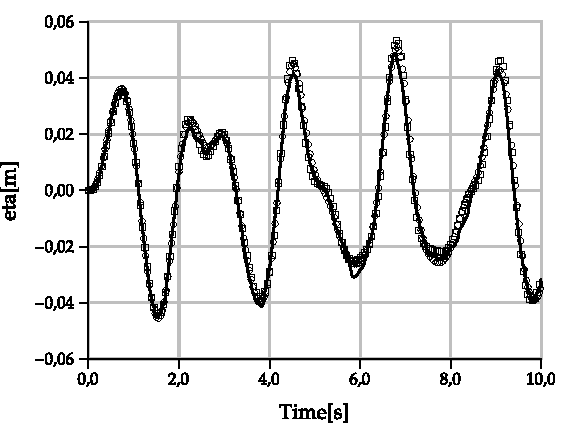
\includegraphics[width=.8\columnwidth]{images/ansari_1.pdf}
    } \\
    %%----segunda subfigura----
    \subfloat[]{
	  \label{fg:ansari-2}         %% Etiqueta para la segunda subfigura
	  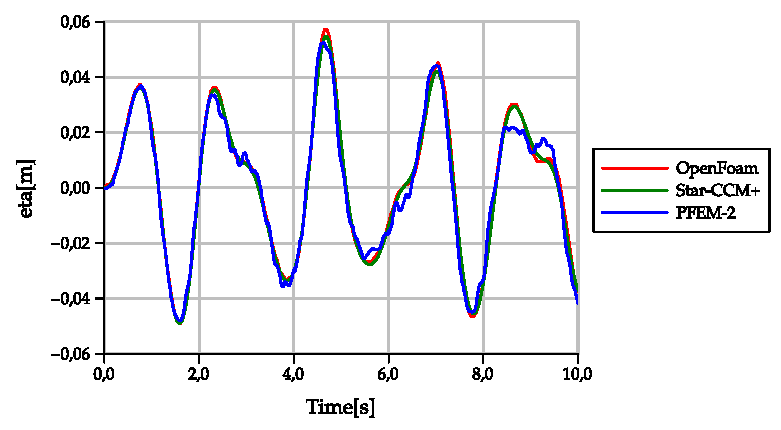
\includegraphics[width=.8\columnwidth]{images/ansari_2.pdf}
    } \\
    \subfloat[]{
	  \label{fg:ansari-3}         %% Etiqueta para la primera subfigura
	  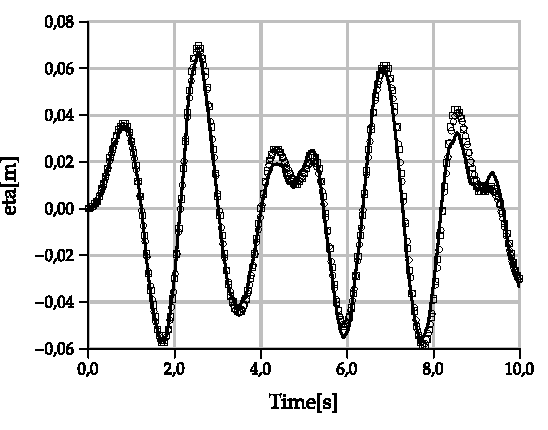
\includegraphics[width=.8\columnwidth]{images/ansari_3.pdf}
    } \\
    %%----segunda subfigura----
    \subfloat[]{
	  \label{fg:ansari-4}         %% Etiqueta para la segunda subfigura
	  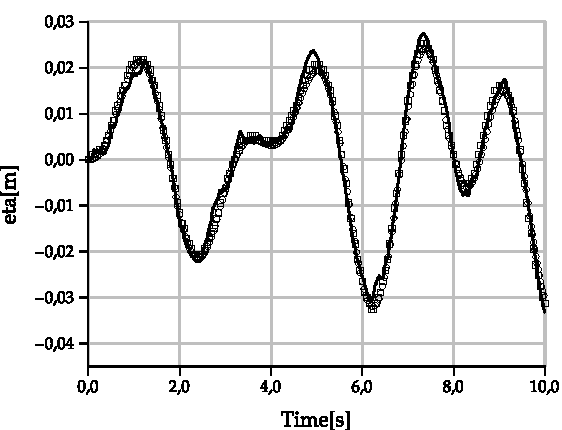
\includegraphics[width=.8\columnwidth]{images/ansari_4.pdf}
    }
   \caption{Sloshing comparison for a two phase flow for different density ratios. Figure \ref{fg:ansari-1}: $\sigma=0.0013$, Figure \ref{fg:ansari-2}: $\sigma=0.05$, Figure \ref{fg:ansari-3}: $\sigma=0.2$ and Figure \ref{fg:ansari-4}: $\sigma=0.8$.
}
   \label{fg:ansari-results}                %% Etiqueta para la figura entera
\end{figure}

Figure \ref{fg:ansari-results} presents results with different density ratios. For each one of them, PFEM-2 simulations shows a good agreement with reference solutions, further more considering that the time step used is around five to ten times bigger.
\clearpage
\subsection{Viscous standing waves}%Re=250,2500.

Computing the dissipation due to wave-breaking remains a challenging problem in the computational fluid mechanics context. In order to analyze the solution with PFEM-2 of two-phase viscous incompressible flows, the evolution of a viscous standing wave has been chosen. This is a classical problem in the scientific literature for which an approximate analytical solution is available for small amplitude perturbations\cite{Lighthill01} and it is of practical interest since it is related to the propagation of gravity waves.

The chosen standing wave configuration consists in a rectangular tank with length $L$ and a water filling height of $H = L/2$. This setup is taken from \cite{Colagrossi12}, and in the Figure \ref{fg:standing-wave-config} a sketch of this configuration is displayed. The wave length is $\lambda = L$, $k$ is the corresponding wave number (i.e. $k = 2\pi/\lambda$), $A$ is the wave amplitude and denotes the ratio $\epsilon=2A/H$.

\begin{figure}[H]
  \begin{center}
      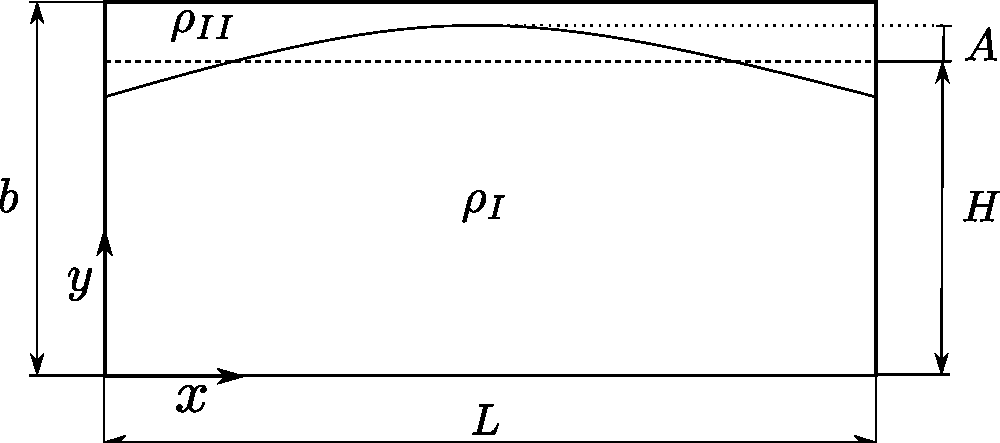
\includegraphics[width=.9\columnwidth]{images/standing_wave.pdf}
  \end{center}
  \caption{\label{fg:standing-wave-config} Configuration scheme of standing wave case. Initial condition is represented by dotted lines. In continuous line is presented an intermediate state where the maximum amplitude $A$ is reached.}
\end{figure}

If the fluid is viscous, the dissipation due to the solid boundary layers is neglected, small-amplitude waves (i.e small $\epsilon$) and small wave steepness (i.e $2A/\lambda \ll 0.1$) are used; an approximate analytical solution of the standing wave evolution can be obtained through the linearization of Navier-Stokes equations for traveling waves:
\begin{align}
 \varphi(x,y,t) & = \varphi_0(x,y)\cos(\omega t) \\
 \varphi_0(x,y) & =-\epsilon\frac{Hg}{2\omega}\frac{\cosh\left[k(y+H)\right]}{\cosh(kH)}\cos(kx)
\end{align}

where the circular frequency $\omega$ is given by the dispersion relation of gravity waves, that is, $\omega^2 = g k \tanh(kH)$ where $g$ is the acceleration of gravity. At time $t = 0$ the free surface is horizontal while the initial fluid velocity is given by $\varphi_0$.

It can be demonstrated that the approximate solution is well posed only for $Re\gg1$ and for $Re^{-1}\ll k \ll Re^{2/3}$, where $Re=H\sqrt{gH}/\nu$ is the Reynolds number for this problem. From that solution, it is possible to obtain the formula that gives the approximate decay of the kinetic energy\cite{Lighthill01}:

\begin{equation}
 \varepsilon_K(t) = \epsilon^2g\frac{\lambda H^2}{32}e^{-4\nu k^2t}\left[1+\cos(2\omega t)\right]
 \label{kin-eq}
\end{equation}

The kinetic attenuation is governed by the coefficient of the exponential $\beta_l = 4\nu k^2$, which depends on the wave number and on the kinematic viscosity $\nu = \mu/\rho_{I}$. Lately work\cite{Antuono13} has demonstrated that generally, the Equation \ref{kin-eq} overestimates the dissipations, especially when the Reynolds number is not very large. Then an improved damping rate is proposed in that paper $\beta = 4\nu k^2 -  2\sqrt{2}k^{11/4}Re^{-3/2}+O(Re^{-2})$, which is next used for comparisons.

To accomplish the linear solution hypothesis, the PFEM-2 simulations have been implemented by using a free-slip condition for the velocity and a Neumann condition for the pressure along each boundary of the tank. Also, the parameters $L=2$, $A=0.05$ and $g=1$ have been selected.

Several Reynolds number ($Re=25,50,250,2500$) have been selected to compare with the approximate analytic dissipation. Problems were solved into a grid with $H/\Delta x=100$ and varying $\Delta t$ in order to solve using a Fourier number $Fo=\frac{\nu\Delta t}{\Delta x^2}$ with a local maximum of $Fo_{max}\approx10-50$. Figure \ref{fg:sw-energy} shows the comparison between the expected dissipation (which includes the improving damping rate) and numerical results with PFEM-2. Large Fourier numbers were used in order to reduce the computation times required to complete the simulations and to show the accuracy of the method working not only with large CFL numbers, even with large diffusion rate.

  \begin{figure}[h]
  \centering
    \subfloat[]{
	  \label{fg:sw-energy-25}
	  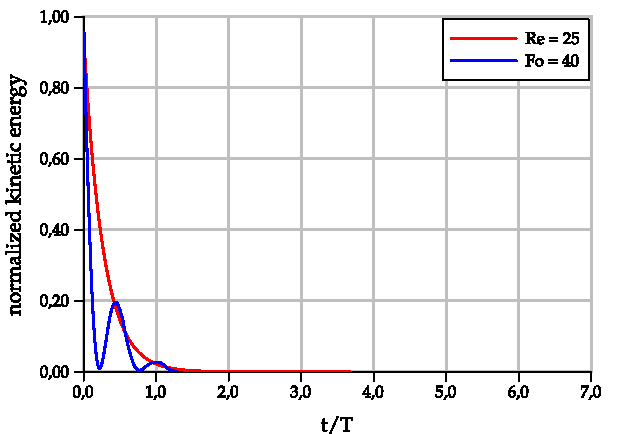
\includegraphics[width=.72\columnwidth]{images/sw_25.pdf}
    } \\
    \subfloat[]{
	  \label{fg:sw-energy-50}
	  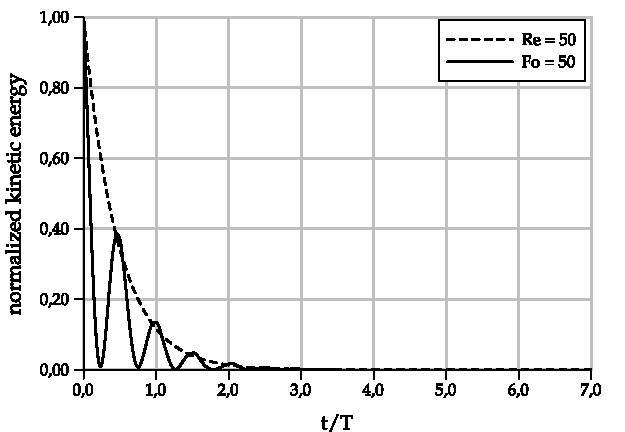
\includegraphics[width=.72\columnwidth]{images/sw_50.pdf}
    } \\
    \subfloat[]{
	  \label{fg:sw-energy-250}
	  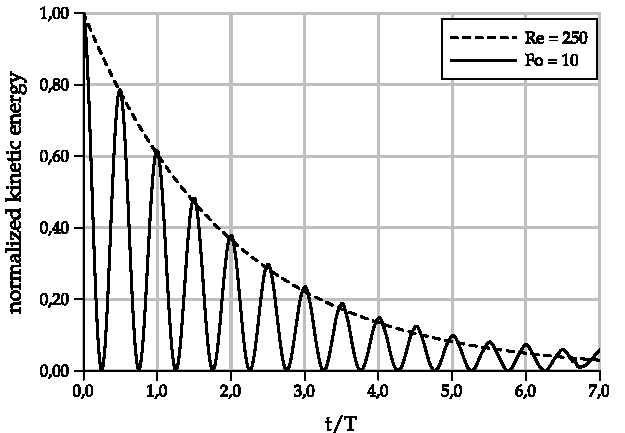
\includegraphics[width=.72\columnwidth]{images/sw_250.pdf}
    } \\
    \subfloat[]{
	  \label{fg:sw-energy-2500}
	  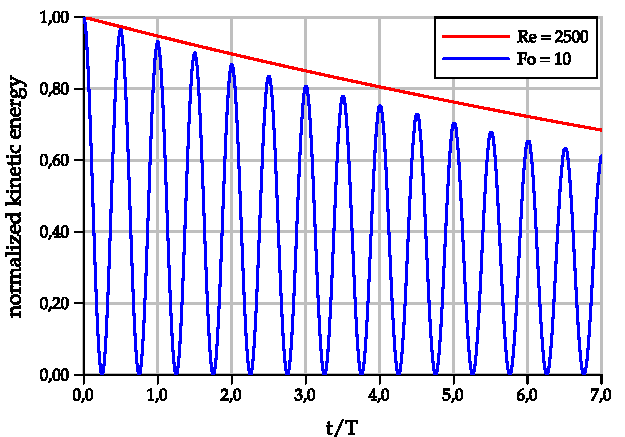
\includegraphics[width=.72\columnwidth]{images/sw_2500.pdf}
    }
   \caption{Kinetic Energy decay for standing wave problem with different Reynolds numbers. Red lines are approximate analytical solutions for total energy and blue lines are numerical solutions with PFEM-2. Reynolds numbers analyzed: $Re=25,50,250,2500$ in Figures \ref{fg:sw-energy-25},\ref{fg:sw-energy-50},\ref{fg:sw-energy-250},\ref{fg:sw-energy-2500} respectively. Legend in each figure indicates the maximum Fourier number used in each numerical simulation.}
   \label{fg:sw-energy}
\end{figure}
% \afterpage{\clearpage}
\subsection{Rayleigh-Taylor Instability}

This problem consists on the evolution of two layers of fluids initially at rest in the gravity field. The top layer is more dense than the one is placed at the bottom. Due to a little disturbance in the contact surface the more dense fluid goes down and the less dense fluid does the opposite. In the intermediate state a mixture is created, which is lately segregated. The final state reaches an stable equilibrium with the more dense fluid at the bottom layer and the less dense fluid at the top layer. The growth and evolution of the instability has been investigated among others by Tryggvason\cite{Tryggvason88} for inviscid incompressible flows, and by Guermond
\& Quartapelle\cite{Guermond00} for viscous flows.

The starting point is the problem documented by Guermond. The domain is $[−d/2,-2d]\times[d/2,2d]$. The initial position of the perturbed interface is $\eta(x) = −0.1d \cos(2\pi x/d)$. The heavy fluid is above and the density ratio is $3$, so that the Atwood
number is $0.5$ according to Tryggvason's definition $At = (\rho_{max}-\rho_{min})/(\rho_{max}+\rho_{min})$. Other physical parameters are selected to obtain $Re=\rho_{min}d^{\frac{3}{2}}g^{\frac{1}{2}}/\mu=1000$. Computational domain is discretized into $160000$ structured triangles ($\Delta x=0.01$) setting slip boundary conditions on each wall. Time step selected is $\Delta t=0.01[s]$, which allows to reach $CFL_{max} \approx 8$.

To compare with reference results, the time is made dimensionless by using $\widetilde{t} = t\sqrt{g\ At}$. Results on the vertical position of the tip of the falling and rising fluid (spike and bubble, respectively) are shown in Figure \ref{fg:rayleigh-rf}. It can be observed that current solution is in good agreement with the reference results.

\begin{figure}[H]
  \begin{center}
      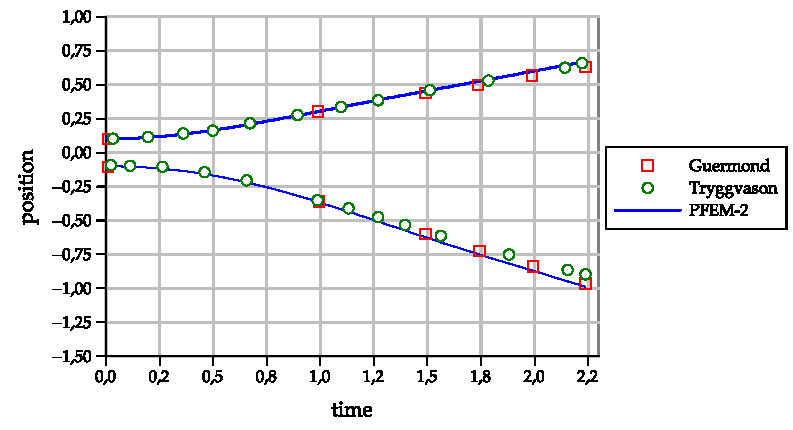
\includegraphics[width=\columnwidth]{images/rayleigh_1.pdf}
  \end{center}
  \caption{\label{fg:rayleigh-rf} Position of rising and falling bubbles versus time. Case with $Re=1000$.}
\end{figure}

On the other hand, the evolution of the instability is shown in Figure \ref{fg:rayleigh-screenshots} at dimensionless times $\widetilde{t}=0, 1, 1.5, 2$. Around $\widetilde{t}=1.5$ the heavy fluid begins to roll up into two counter-rotating vortices. Later, around $\widetilde{t} = 2$, these two vortices become unstable and a pair of secondary vortices appear at the tails of the roll-ups. These shapes of the fluid interface obtained with PFEM-2 are similar than those of the reference results.


\begin{figure}[htbp]
  \begin{center}
      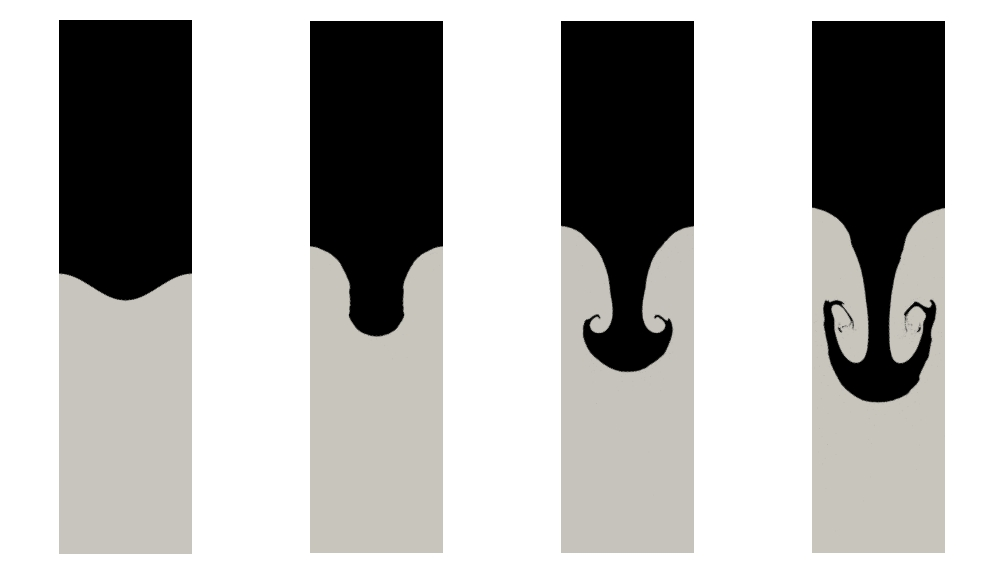
\includegraphics[width=\columnwidth]{images/rayleigh_2.jpg}
  \end{center}
  \caption{\label{fg:rayleigh-screenshots} Rayleigh-Taylor instability evolution. Case with $Re=1000$. From left to right $\widetilde{t} =0.0$, $1.0$, $1.5$, $2.0$.}
\end{figure}
\afterpage{\clearpage}
\subsection{Sloshing roll.}%ETSIN experimental tests

\subsection{Dam-break problem}%ETSIN experimental tests

The objectives of this section are to compare experimental measurements on dam-break flow over a dry horizontal bed with the numerical approximation carried out with the pfem algorithm. The extensive set of experimental data is extracted from \cite{Lobovsky13}, where the dynamics of the dam break wave impacting a vertical wall downstream the dam, with emphasis on the pressure loads and surface evolution after the dam burst, are presented.

Computational configuration of the tank used in experimental cases is presented in Figure \ref{fg:dambreak-config}. There, the locations of water level measuring points and pressure sensors are shown. In this report only the case with $H=300[mm]$ is analyzed. Two-phase non-viscous flow simulation is carried on, with $\rho_{water}=1000[kg/m^3]$ and $\rho_{air}=1[kg/m^3]$ with a gravity force $\mathbf{g}=-10\ \hat{j} [m/s^2]$. The 2D computational grid used has $322\times120$ nodes, conforming a mesh with around $80000$ triangles. Boundary conditions are slip on all walls, and $\Delta t$ is fixed to $0.1$, which allows to reach $CFL_{max}\approx20$ when free surface impacts the downstream wall.

\begin{figure}[htbp]
  \begin{center}
      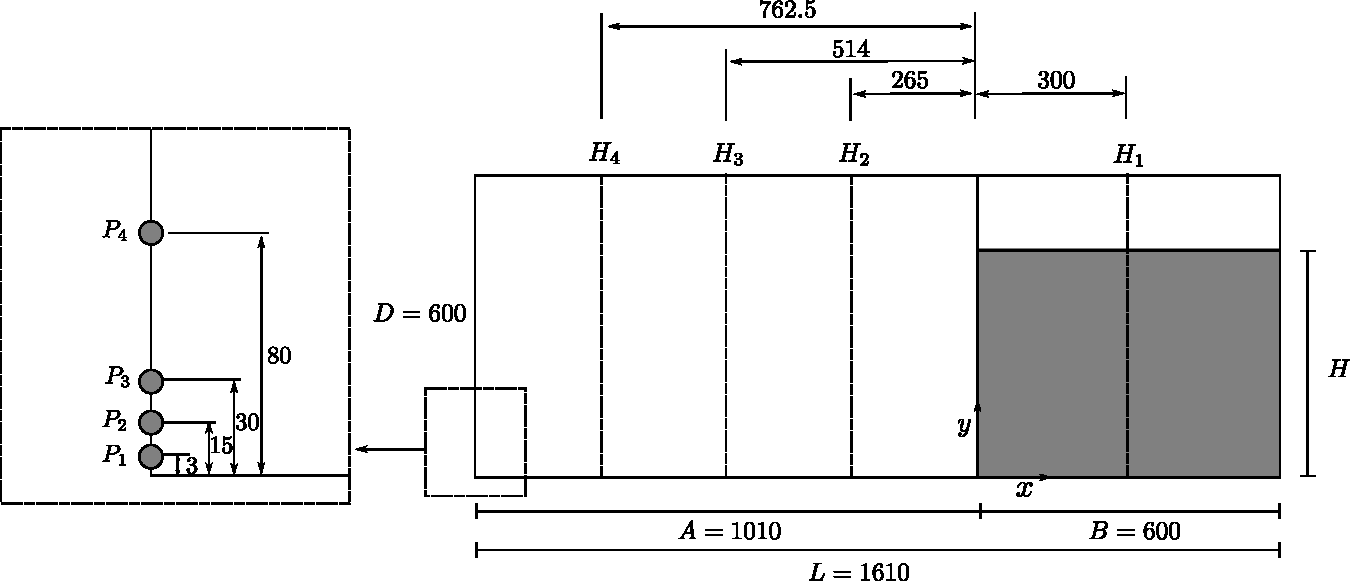
\includegraphics[width=\columnwidth]{images/dam_break_config.pdf}
  \end{center}
  \caption{\label{fg:dambreak-config} Configuration scheme of the dam-break case. $H_1$, $H_2$, $H_3$, $H_4$ present the locations of water level measuring positions. Also, $P_1$, $P_2$, $P_3$, $P_4$ show the locations of pressure sensors at the impact wall downstream the dam. Grey zone represents the initial condition. Dimensions in millimeters.}
\end{figure}

Figure \ref{fg:dambreak-h} shows the comparison between experimental and numerical results for each water-level measurement. A good agreement can be observed, moreover taken into account the capture of the back wave and splashing start events.
  \begin{figure}[h]
  \centering
    \subfloat[]{
	  \label{fg:dambreak-h1}         %% Etiqueta para la primera subfigura
	  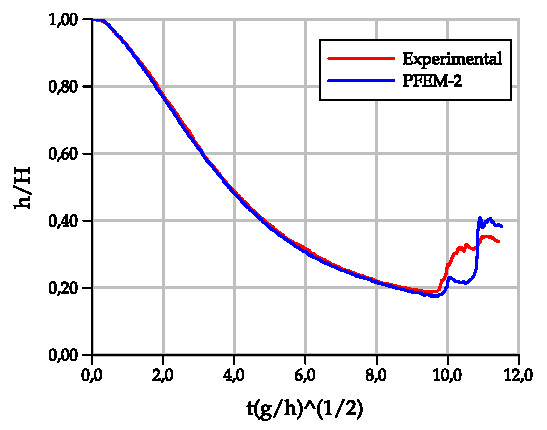
\includegraphics[width=.48\columnwidth]{images/dambreak_h1.pdf}
    }
    %%----segunda subfigura----
    \subfloat[]{
	  \label{fg:dambreak-h2}         %% Etiqueta para la segunda subfigura
	  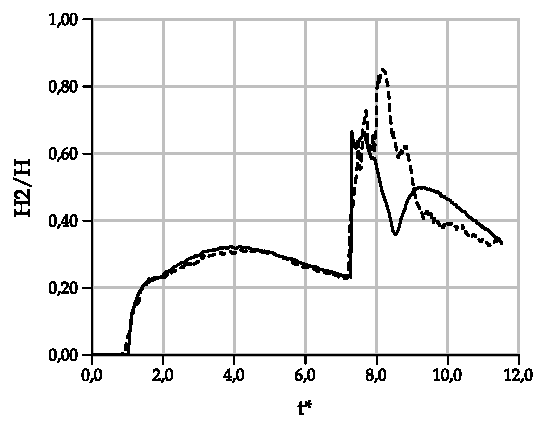
\includegraphics[width=.48\columnwidth]{images/dambreak_h2.pdf}
    } \\
    \subfloat[]{
	  \label{fg:dambreak-h3}         %% Etiqueta para la primera subfigura
	  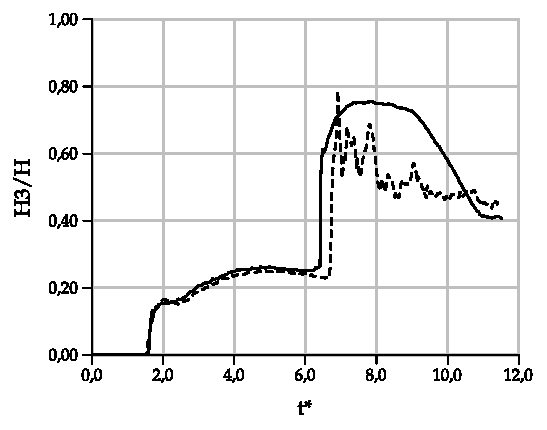
\includegraphics[width=.48\columnwidth]{images/dambreak_h3.pdf}
    }
    %%----segunda subfigura----
    \subfloat[]{
	  \label{fg:dambreak-h4}         %% Etiqueta para la segunda subfigura
	  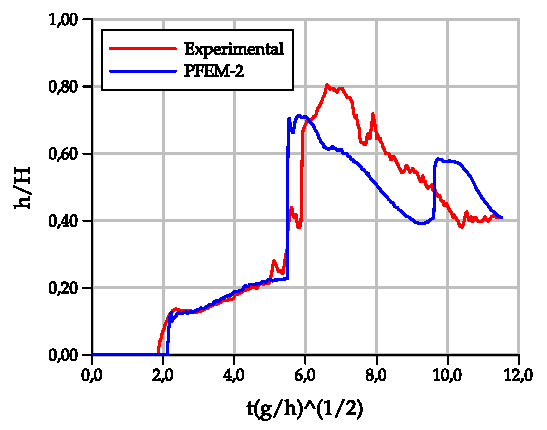
\includegraphics[width=.48\columnwidth]{images/dambreak_h4.pdf}
    }
   \caption{Water level elevations at locations $H_1$, $H_2$, $H_3$ and $H_4$ for tests with $H=300[mm]$ initial filling height compared to data from literature experimental results\cite{Lobovsky13} and numerical results with PFEM-2.}
   \label{fg:dambreak-h}                %% Etiqueta para la figura entera
\end{figure}

The impact pressure was measured with four sensors at the vertical wall at the end of the downstream flume, as described in Figure \ref{fg:dambreak-config}. The statistical analysis of the pressure peaks, rise times and the occurrence time, i.e. the time between
the opening of the dam gate and the occurrence of the impact, is presented in Figure \ref{fg:dambreak-p}. The shown pressure $P$ is non-dimensionalized with regards to the hydrostatic pressure at the bottom of the reservoir and denoted as $P^∗$.

In the reference work, the analysis is focused on peaks events. It can be noticed that the highest peak is recorded by sensor number 1 which is the sensor receiving the full impact, whilst the pressure of the other sensors is given by the run up of the flow. It can also be observed that sensor number 4, i.e. the sensor located at the highest position, does not show a pure impact event, see Figure \ref{fg:dambreak-p4}, and actually the maximum for this sensor is obtained later in time, when the water falls back after running along the wall. Numerical solution behavior follows the mentioned conclusions, but the pressure values are not between the statistical limits of experimental data. Also, a discrepancy can be observed with the peaks times for sensors $1$ to $3$. This difference can be assigned to the numerical simplification which does not model the gate movement.

  \begin{figure}[h]
  \centering
    \subfloat[]{
	  \label{fg:dambreak-p1}         %% Etiqueta para la primera subfigura
	  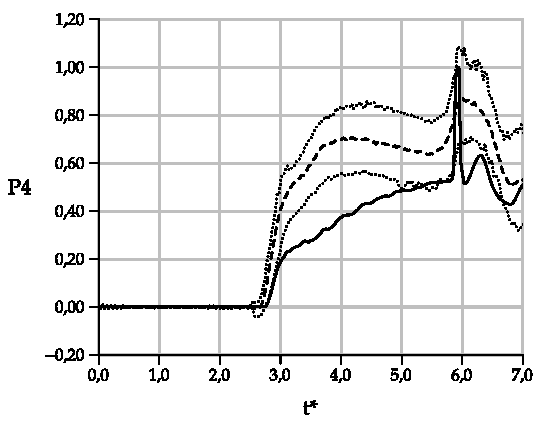
\includegraphics[width=.48\columnwidth]{images/dambreak_p4.pdf}
    }
    %%----segunda subfigura----
    \subfloat[]{
	  \label{fg:dambreak-p2}         %% Etiqueta para la segunda subfigura
	  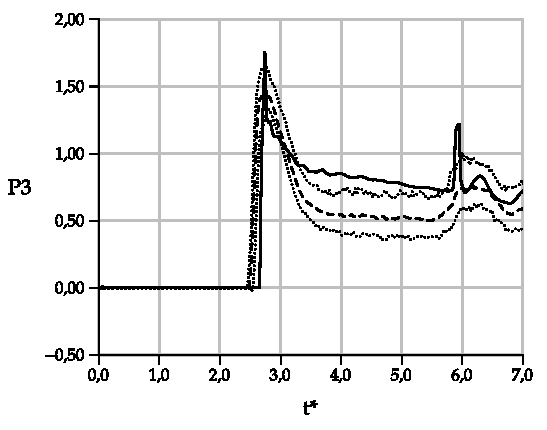
\includegraphics[width=.48\columnwidth]{images/dambreak_p3.pdf}
    } \\
    \subfloat[]{
	  \label{fg:dambreak-p3}         %% Etiqueta para la primera subfigura
	  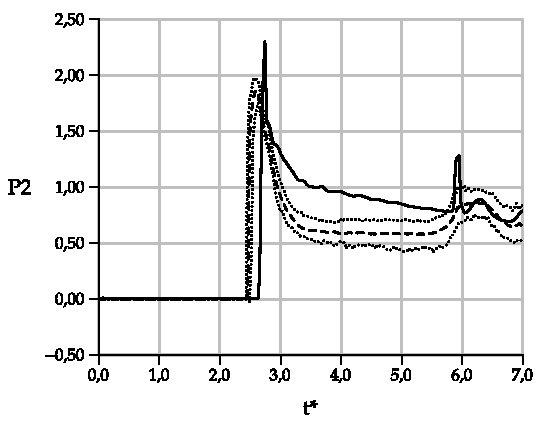
\includegraphics[width=.48\columnwidth]{images/dambreak_p2.pdf}
    }
    %%----segunda subfigura----
    \subfloat[]{
	  \label{fg:dambreak-p4}         %% Etiqueta para la segunda subfigura
	  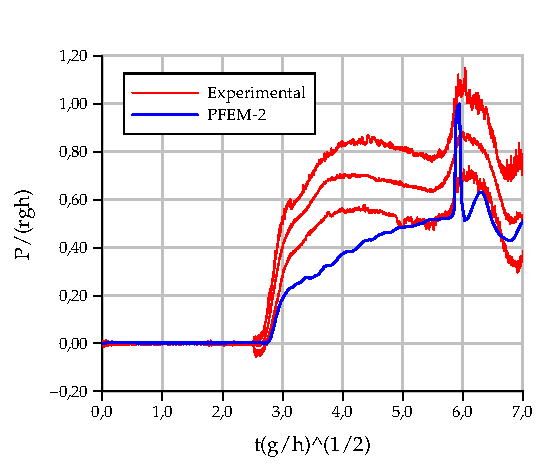
\includegraphics[width=.48\columnwidth]{images/dambreak_p1.pdf}
    }
   \caption{Pressure time histories comparison between experimental results\cite{Lobovsky13} and numerical results with PFEM-2. Locations $P_1$, $P_2$, $P_3$, $P_4$ area presented in Figures \ref{fg:dambreak-p1},\ref{fg:dambreak-p2},\ref{fg:dambreak-p3},\ref{fg:dambreak-p4} respectively. Experimental results shows the median and percentiles $2.5$ and $97.5$.}
   \label{fg:dambreak-p}                %% Etiqueta para la figura entera
\end{figure}

  \begin{figure}[H]
  \centering
    \subfloat[]{
	  \label{fg:dambreak-1}
	  
\includegraphics[width=.48\columnwidth]{images/dambreak_pfem_1.jpg}
    }
    %%----segunda subfigura----
    \subfloat[]{
	  \label{fg:dambreak-2}
	  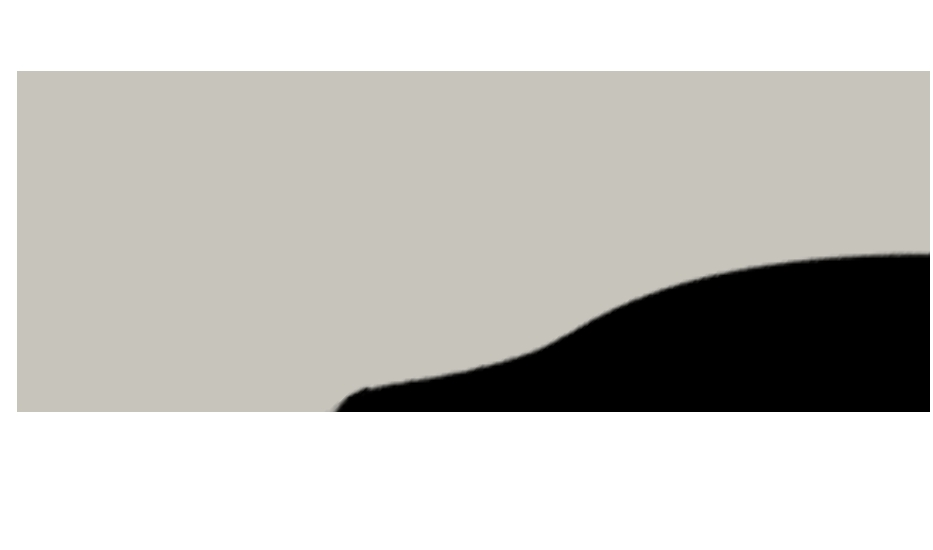
\includegraphics[width=.48\columnwidth]{images/dambreak_pfem_2.jpg}
    } \\
    \subfloat[]{
	  \label{fg:dambreak-3}
	  
\includegraphics[width=.48\columnwidth]{images/dambreak_pfem_3.jpg}
    }
    %%----segunda subfigura----
    \subfloat[]{
	  \label{fg:dambreak-4}
	  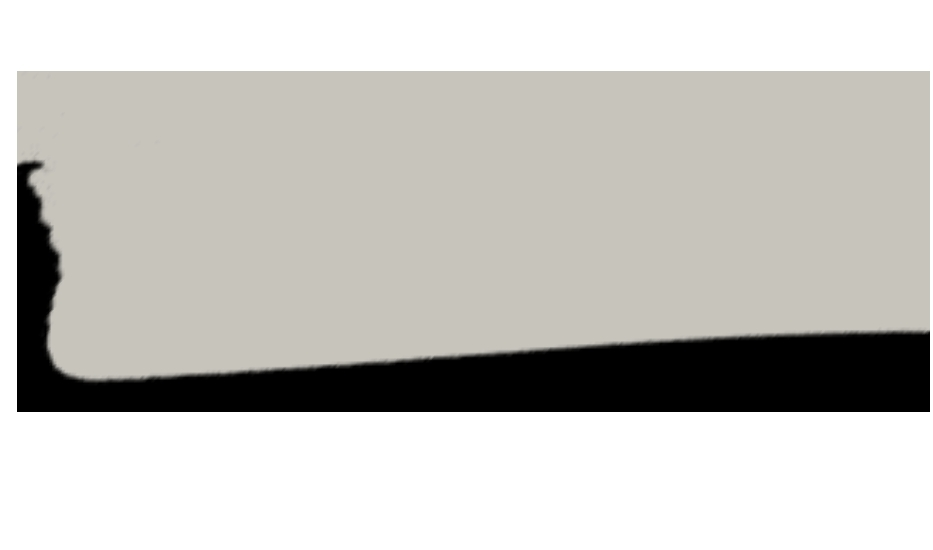
\includegraphics[width=.48\columnwidth]{images/dambreak_pfem_4.jpg}
    }\\
        \subfloat[]{
	  \label{fg:dambreak-5}
	  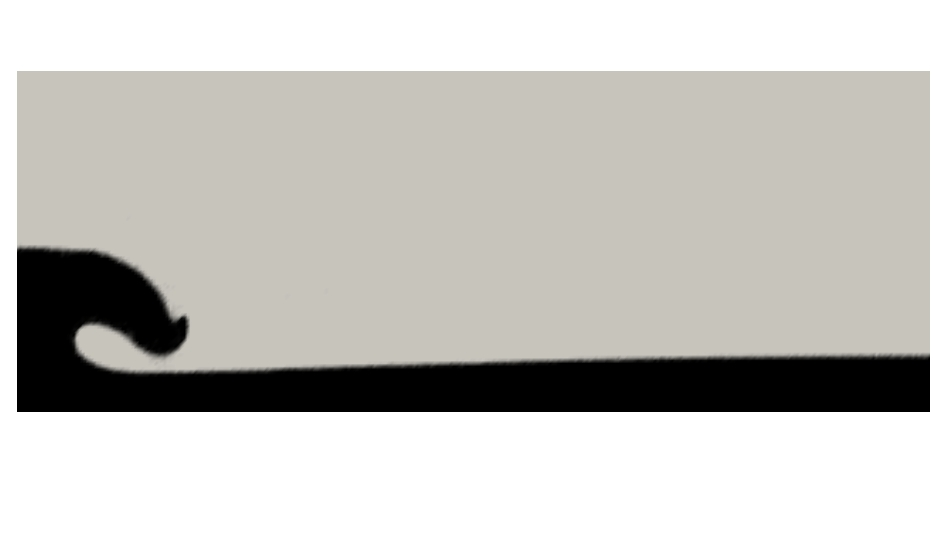
\includegraphics[width=.48\columnwidth]{images/dambreak_pfem_5.jpg}
    }
    %%----segunda subfigura----
    \subfloat[]{
	  \label{fg:dambreak-6}
	  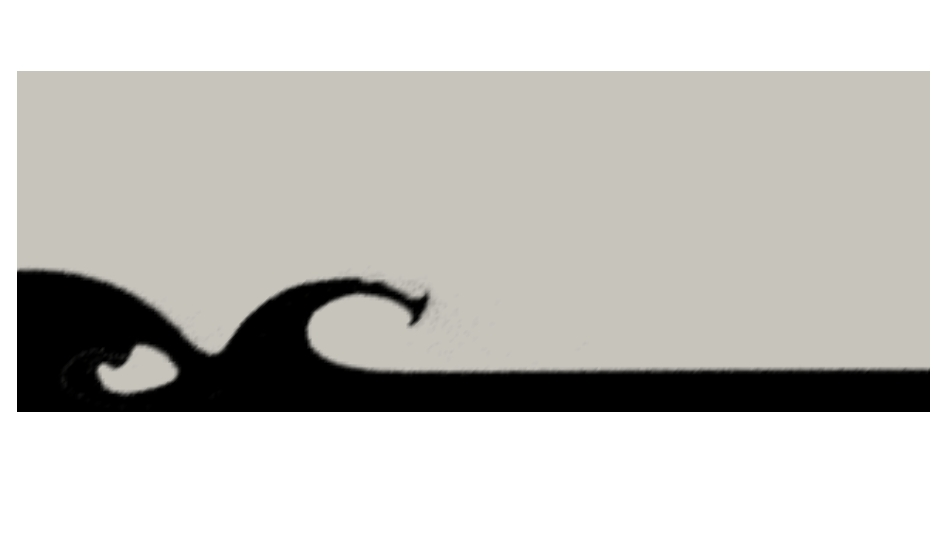
\includegraphics[width=.48\columnwidth]{images/dambreak_pfem_6.jpg}
    } \\
    \subfloat[]{
	  \label{fg:dambreak-7}
	  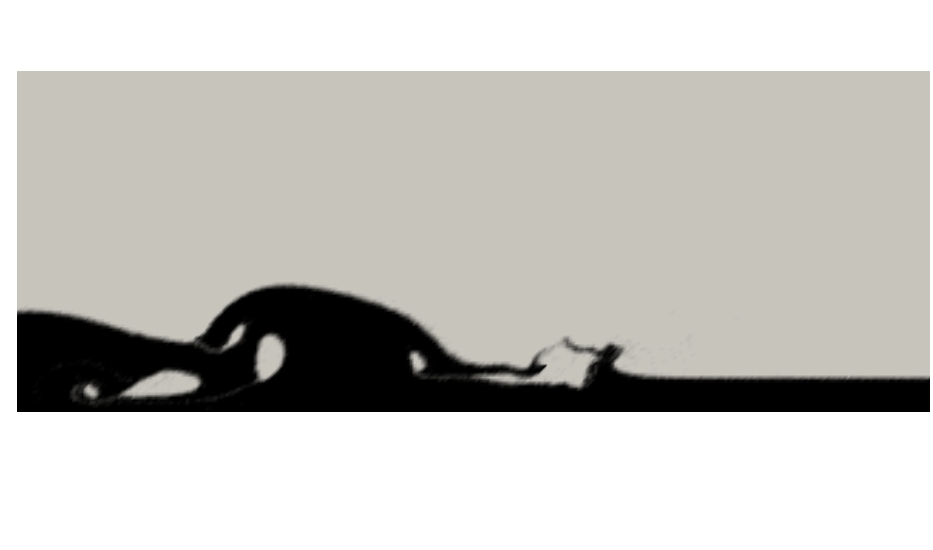
\includegraphics[width=.48\columnwidth]{images/dambreak_pfem_7.jpg}
    }
    %%----segunda subfigura----
    \subfloat[]{
	  \label{fg:dambreak-8}
	  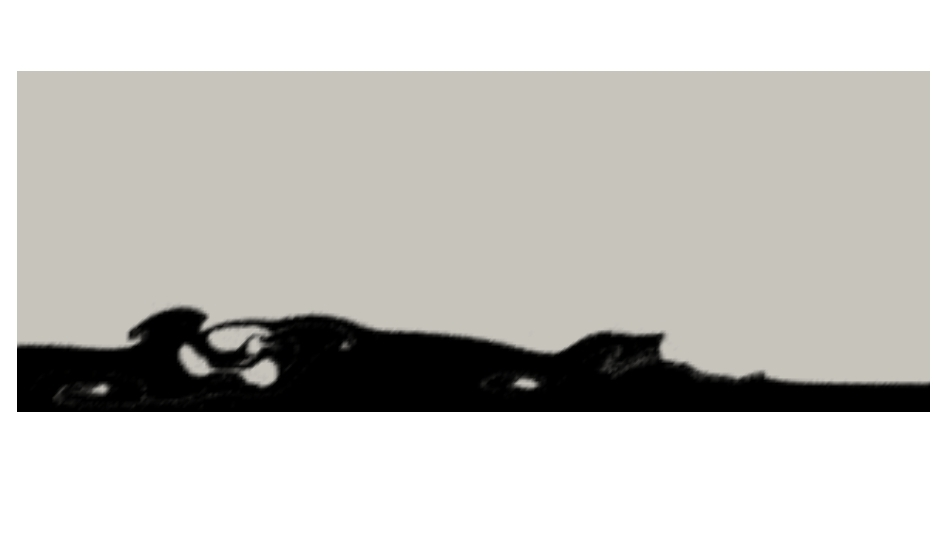
\includegraphics[width=.48\columnwidth]{images/dambreak_pfem_8.jpg}
    }
   \caption{Snapshots of the dam-break at times $t=0,0.25,0.5,0.75,1,1.25,1.5,1.75[s]$.}
   \label{fg:dambreak-screenshots}
\end{figure}
\clearpage
% \subsection{Shear layer flow.}



\section{Conclusion}



% use section* for acknowledgement
\section*{Acknowledgment}
% optional entry into table of contents (if used)
%\addcontentsline{toc}{section}{Acknowledgment}
The research  leading  to these results has received funding from the Spanish Ministry for Science and
 Innovation under the grant TRA2010-16988
``Caracterizaci\'on Num\'erica y Experimental de las Cargas Fluido-Din\'amicas en el transporte de Gas Licuado''.
All the authors want to thank Mr. Hugo Gee for proof-reading the paper.

\bibliographystyle{plain}
\bibliography{mybib}

% \begin{thebibliography}{99}
%
% \bibitem{HoodTaylor73}
% P.~Hood and C.~Taylor, \emph{Numerical solution of the Navier–Stokes equations using the finite
% element technique}, Comput. Fluids, 1:1–28, 1973.
%
% \bibitem{Idelsohn12b}
% S.R. Idelsohn, N.M. Nigro, J.M. Gimenez, R. Rossi and J. Marti, \emph{A fast and accurate method to solve the incompressible Navier-Stokes equations}, Engineering Computations, 30-Iss:2:197-222, 2013.
%
% \bibitem{Lobovsky13}
% L. Lobovsky, E. Botia-Vera, F. Castellana, J. Mas-Soler and A. Souto-Iglesias , \emph{Experimental investigation of dynamic pressure loads during dam break}, Journal of Fluids and Structures, submitted, 2013.
%
% % \bibitem{Strubelj11}
% % L. Strubelj and I. Tiselj, \emph{Two-fluid model with interface sharpening}, Int. J. Numer. Meth. Engng, 85:575–590, 2011
%
% \bibitem{Osher01}
% S.J. Osher and R.P. Fedkiw, \emph{Level set methods: an overview and some recent results}, Journal of Computational Physics, 169:463–502, 2001
%
% \bibitem{Goni13}
% Jes\'us G\'omez-Go\~ni, Carlos A. Garrido-Mendoza, Jos\'e Luis Cerc\'os and Leo Gonz\'alez, \emph{Two phase analysis of sloshing in a rectangular container with Volume of Fluid (VOF) methods}, Ocean Engineering 73:208–212, 2013
%
% \bibitem{Guermond00}
% J.L. Guermond and L. Quartapelle, \emph{A Projection FEM for Variable Density Incompressible Flows}, Journal of Computational Physics 165, 167–188, 2000.
%
% \bibitem{Tryggvason88}
% G. Tryggvason, \emph{Numerical Simulations of the Rayleigh-Taylor Instability}, Journal of Computational Physics 75, 253-282, 1988.
%
% \bibitem{Lighthill01}
% J. Lighthill, \emph{Waves in fluids}, Cambridge University Press, 2001.
%
% \bibitem{Colagrossi12}
% A. Colagrossi, A. Souto-Iglesias, M. Antuono and S. Marrone, \emph{Modeling of gravity wave viscous attenuation}, 7th international SPHERIC workshop, Prato-Italy, 2012.
%
%
%
% \end{thebibliography}


% that's all folks
\end{document}


